\documentclass[12pt]{article}
\usepackage{amsfonts, epsfig, graphicx}

\title{Field Manual for LWA Deployment}
\author{Cherie Day}
\date{2-20-2015}

\begin{document}
\maketitle

\center
{\bf Introduction} \\
This document is a set of instructions for constructing the LWA antenna for field deployment. Adapted from \underline{Complete Guide to Antenna Assembly LWA Engineering Memo ARR0005} by Chenoa Tramblay, Steven Tremblay and Joe Craig (5-21-2011).

\tableofcontents

\newpage

\begin{enumerate}

\section{Ground Screen Fabrication} \label{GNDscreenFabSec}
	\subsection{Required Tools}
		\begin{itemize}
			\item 2 People
			\item Bolt-cutters
			\item Nicopress crimping tool
		\end{itemize}
	\subsection{Required Materials}
		\begin{itemize}
			\item 6ft x 200ft Ground Screen Rolls (4 inch squares)
			\item Nicross splice sleeves (6 for every 10 ft section)
			\item Pieces of board/wood (optional)
		\end{itemize}
	\subsection{Prerequisite Tasks}
		\begin{itemize}
			\item None.
		\end{itemize}
	\subsection{Procedure}
		\begin{enumerate}
			\item \emph{Unroll the ground screen} \\ Unroll two of the rolls of ground screen and overlap them by 2ft to create a 10ft x 10ft square. See Figure \ref{Grid} for how this should look. A piece of wood can be used to secure the ends and prevent the screen from rolling up while it is being worked on.
			\item \emph{Cut out the screen} \\ Once the overlap is aligned, the screen can be cut into 10 ft sections. The recommended procedure is to cut out a full square so the screen won't have wire protruding from the edge. Cut the screen using either bolt-cutters or dykes and make sure there are no sharp edges once the cutting is complete.
			\item \emph{Crimp on splice sleeves on the ground screen} \\ 6 nicopress splice sleeves are used for every 10 ft section. 2 sleeves are placed on each edge, one on each side of the overlap, and 2 in the middle on each side of the overlap (See Figure \ref{Grid}). They are crimped with the Nicopress tool.
			\item \emph{Carry the screen to a mast or set aside} \\ When each section is complete, it can be rolled easily and carried out to each antenna location or put aside until needed.
		\end{enumerate}
		
\begin{figure}[!h]
	\center
	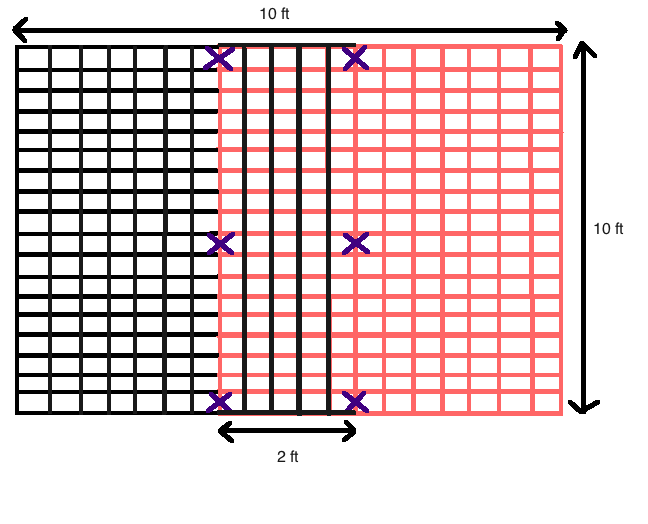
\includegraphics[width=\linewidth]{plots/GroundScreenGrid.png}
	\caption{Line drawing of a fabricated ground screen. Each square is 4in. and the total final screen is 10ft x 10 ft. The splice sleeves that connect the two pieces are placed in the position of the big X, for a total of 6 sleeves. \label{Grid}}
\end{figure}


\section{Triangle Assembly} \label{TriAssemSec}
	\subsection{Required Tools}
		\begin{itemize}
			\item 1 Person
			\item 5/16 Socket Wrench
			\item 5/32 Allen Wrench
			\item Optional: Phillips-head screwdriver
		\end{itemize}

	\subsection{Required Materials}
		\begin{itemize}
			\item Four Triangles
			\item Center Flange (Part No. LWA10-107)
			\item 10-32 UNF X 1.25 hex SEM SCREW, 18-8 S.S. (Part No. LWA10-130)
			\item 5/16-18 UNC X 1/2 Hex Set Screw, 18-8 S.S. (Part No. LWA10-131)
		\end{itemize}

		\subsection{Prerequisite Tasks}
			\begin{itemize}
				\item None.
			\end{itemize}
			
	\subsection{Procedure}
		\begin{enumerate}
			\item Gather the 4 pre-constructed triangles and the center flange (Figure \ref{TriHalfDone})
			\item Use the hex wrench to put the set screws in the underside of the center flange (the extended side, not the flat side). \\ \emph{Warning: \bf}Overtightening will cause difficulties in fitting the center flange over the antenna mast.
			\item Place the center flange on a flat surface with the flat side up. Take one of the triangles and align the corner with the two holes for bolts with two of the center flange holes, making sure that the sloped side of the other two corners faces up. Lightly put the two screws in. Tightening before both are in might cause one or both to not fit.
			\item Tighten evenly so that they both fit on the flange using a 5/16 socket wrench or a Phillps-head screwdriver. (Figure \ref{TriHalfDone}) \\ \emph{Warning: \bf}To avoid stripping the bolts, do not use an electric wrench.
			\item Repeat the last 2 steps with the three remaining triangles, making sure all four are fully tightened. See Figures \ref{TriComplete} and \ref{TriZoom}.

		\end{enumerate}

\begin{figure}[!hp]
  \center
     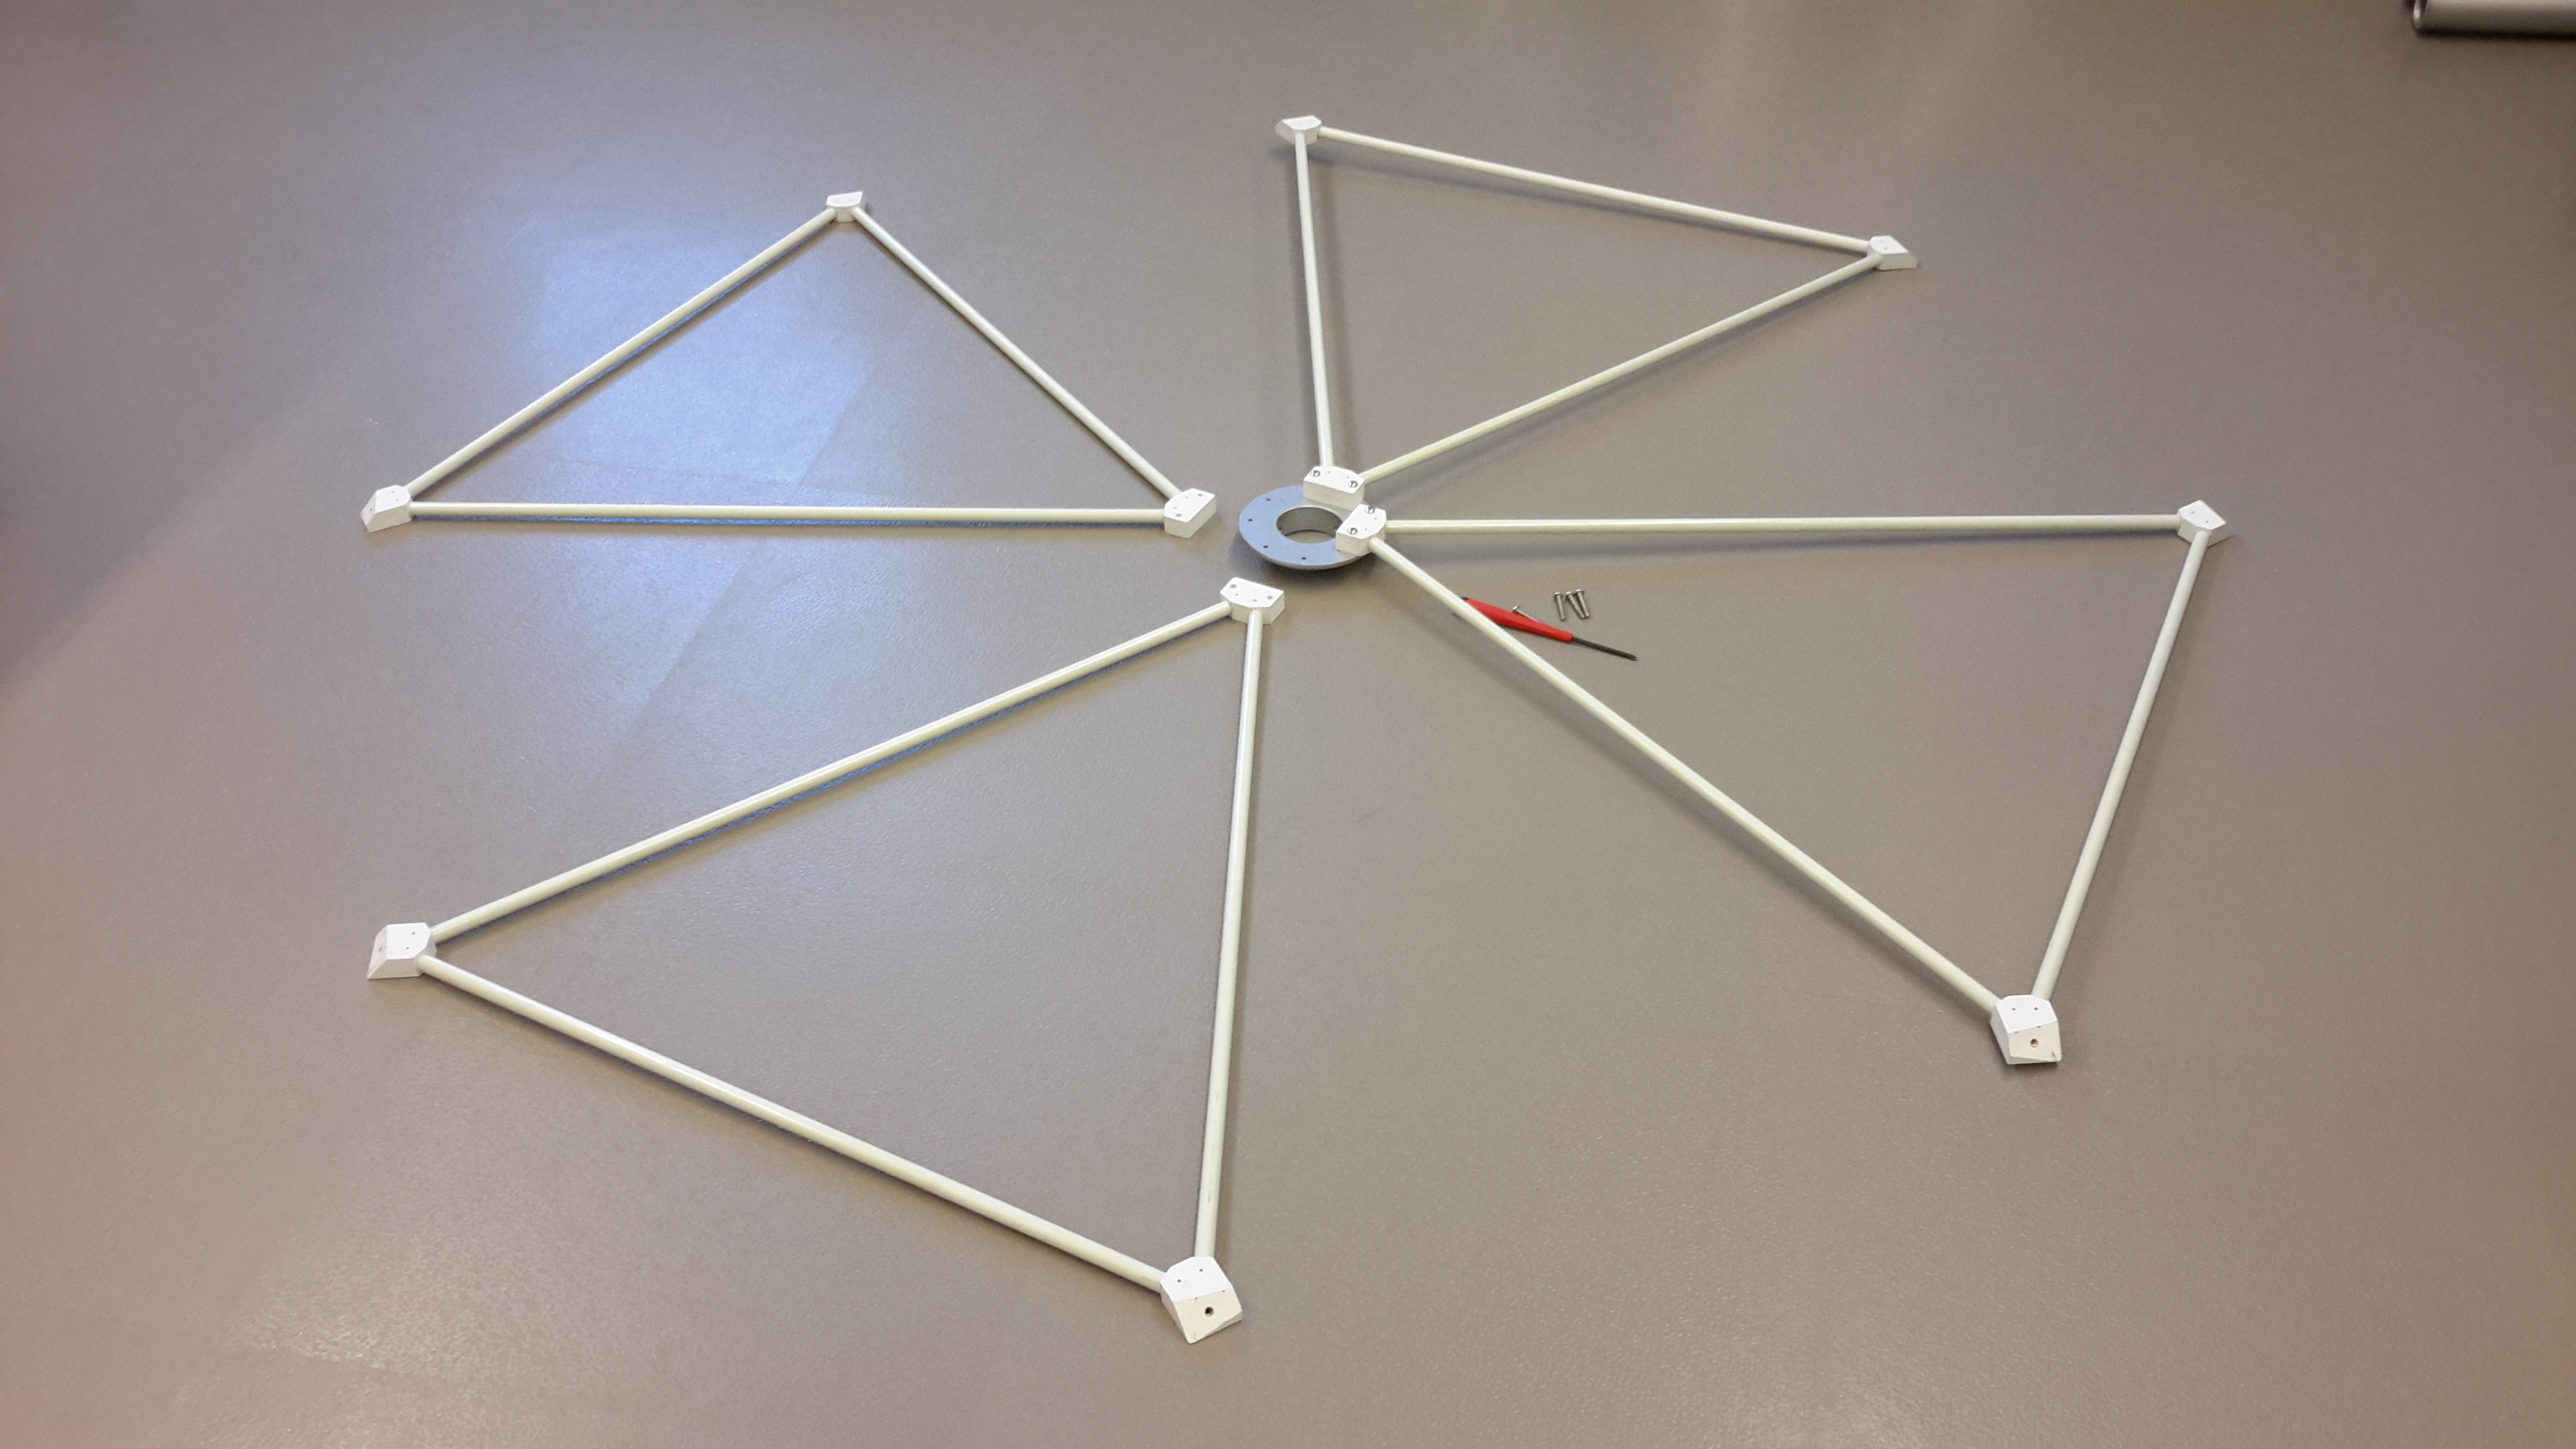
\includegraphics[width=\linewidth]{plots/20141125_095619.jpg}
     \caption{The center flange and four triangles (sloped corners pointing up). Partially constructed. \label{TriHalfDone}}
\end{figure}

\begin{figure}[!hp]
   \center
     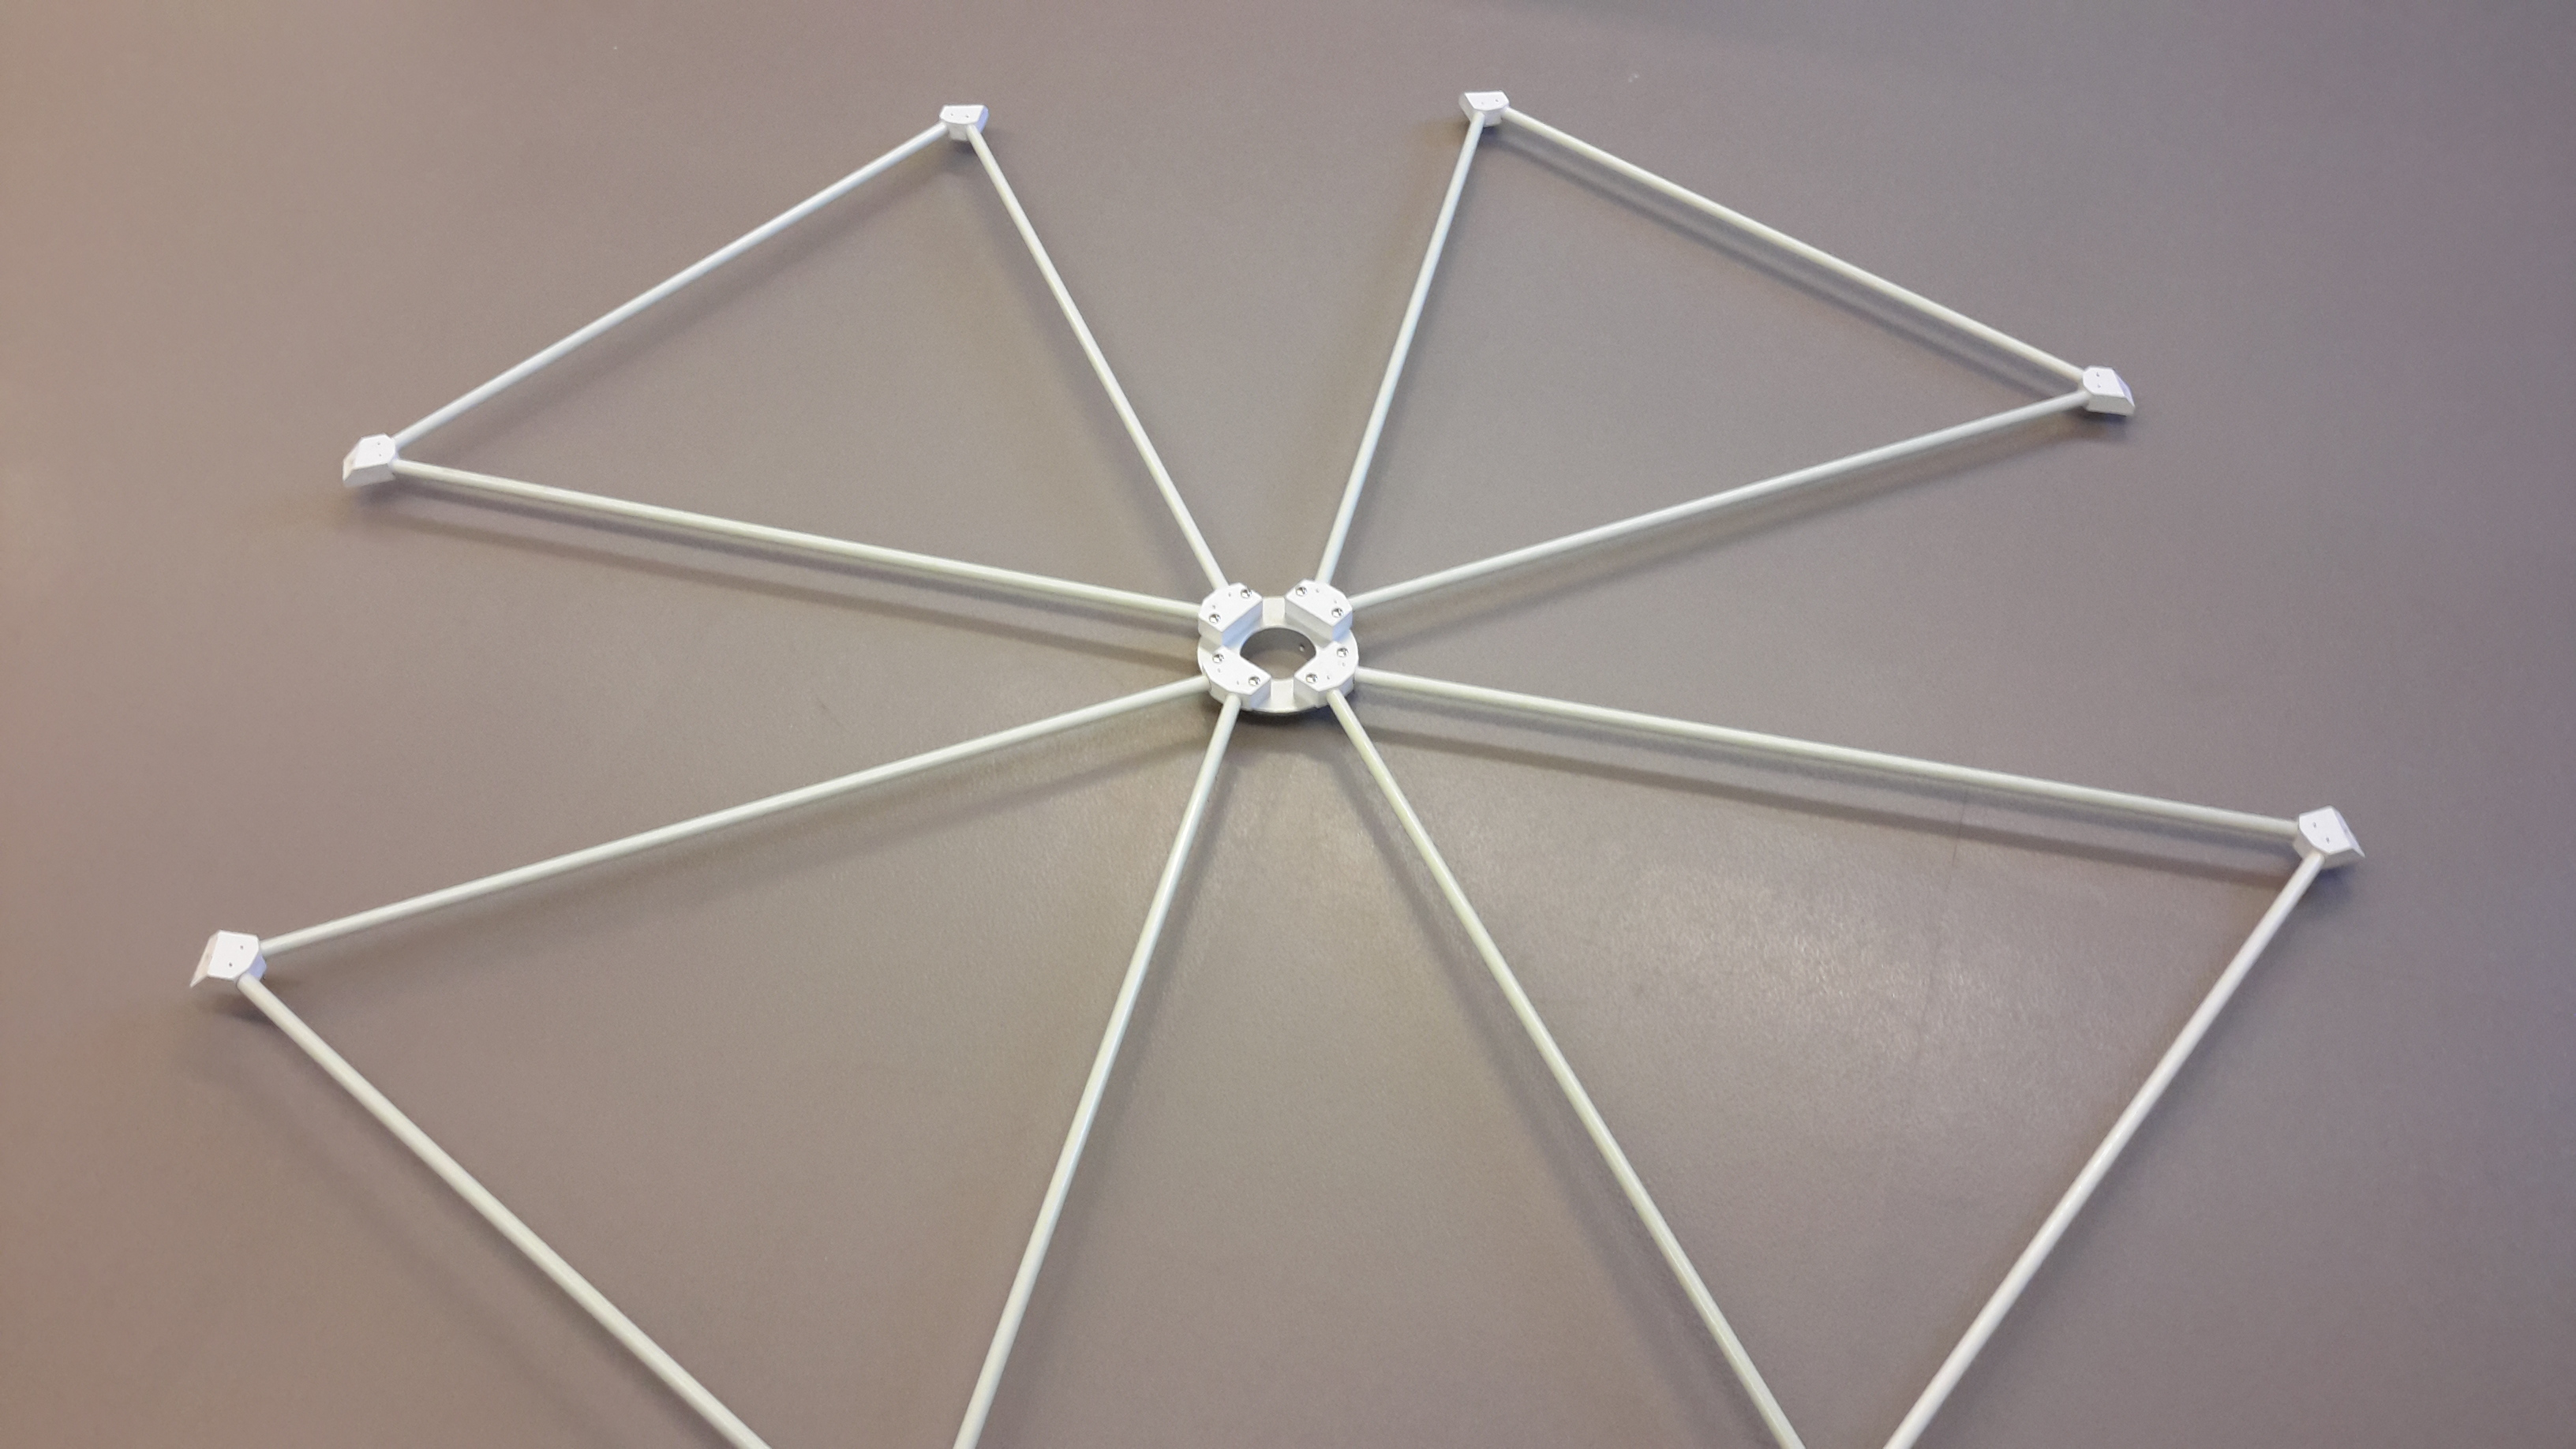
\includegraphics[width=\linewidth]{plots/20141125_100039.jpg}
        \caption{Fully constructed triangle assembly. \label{TriComplete}}
\end{figure}

\begin{figure}[!tp]
  \center
    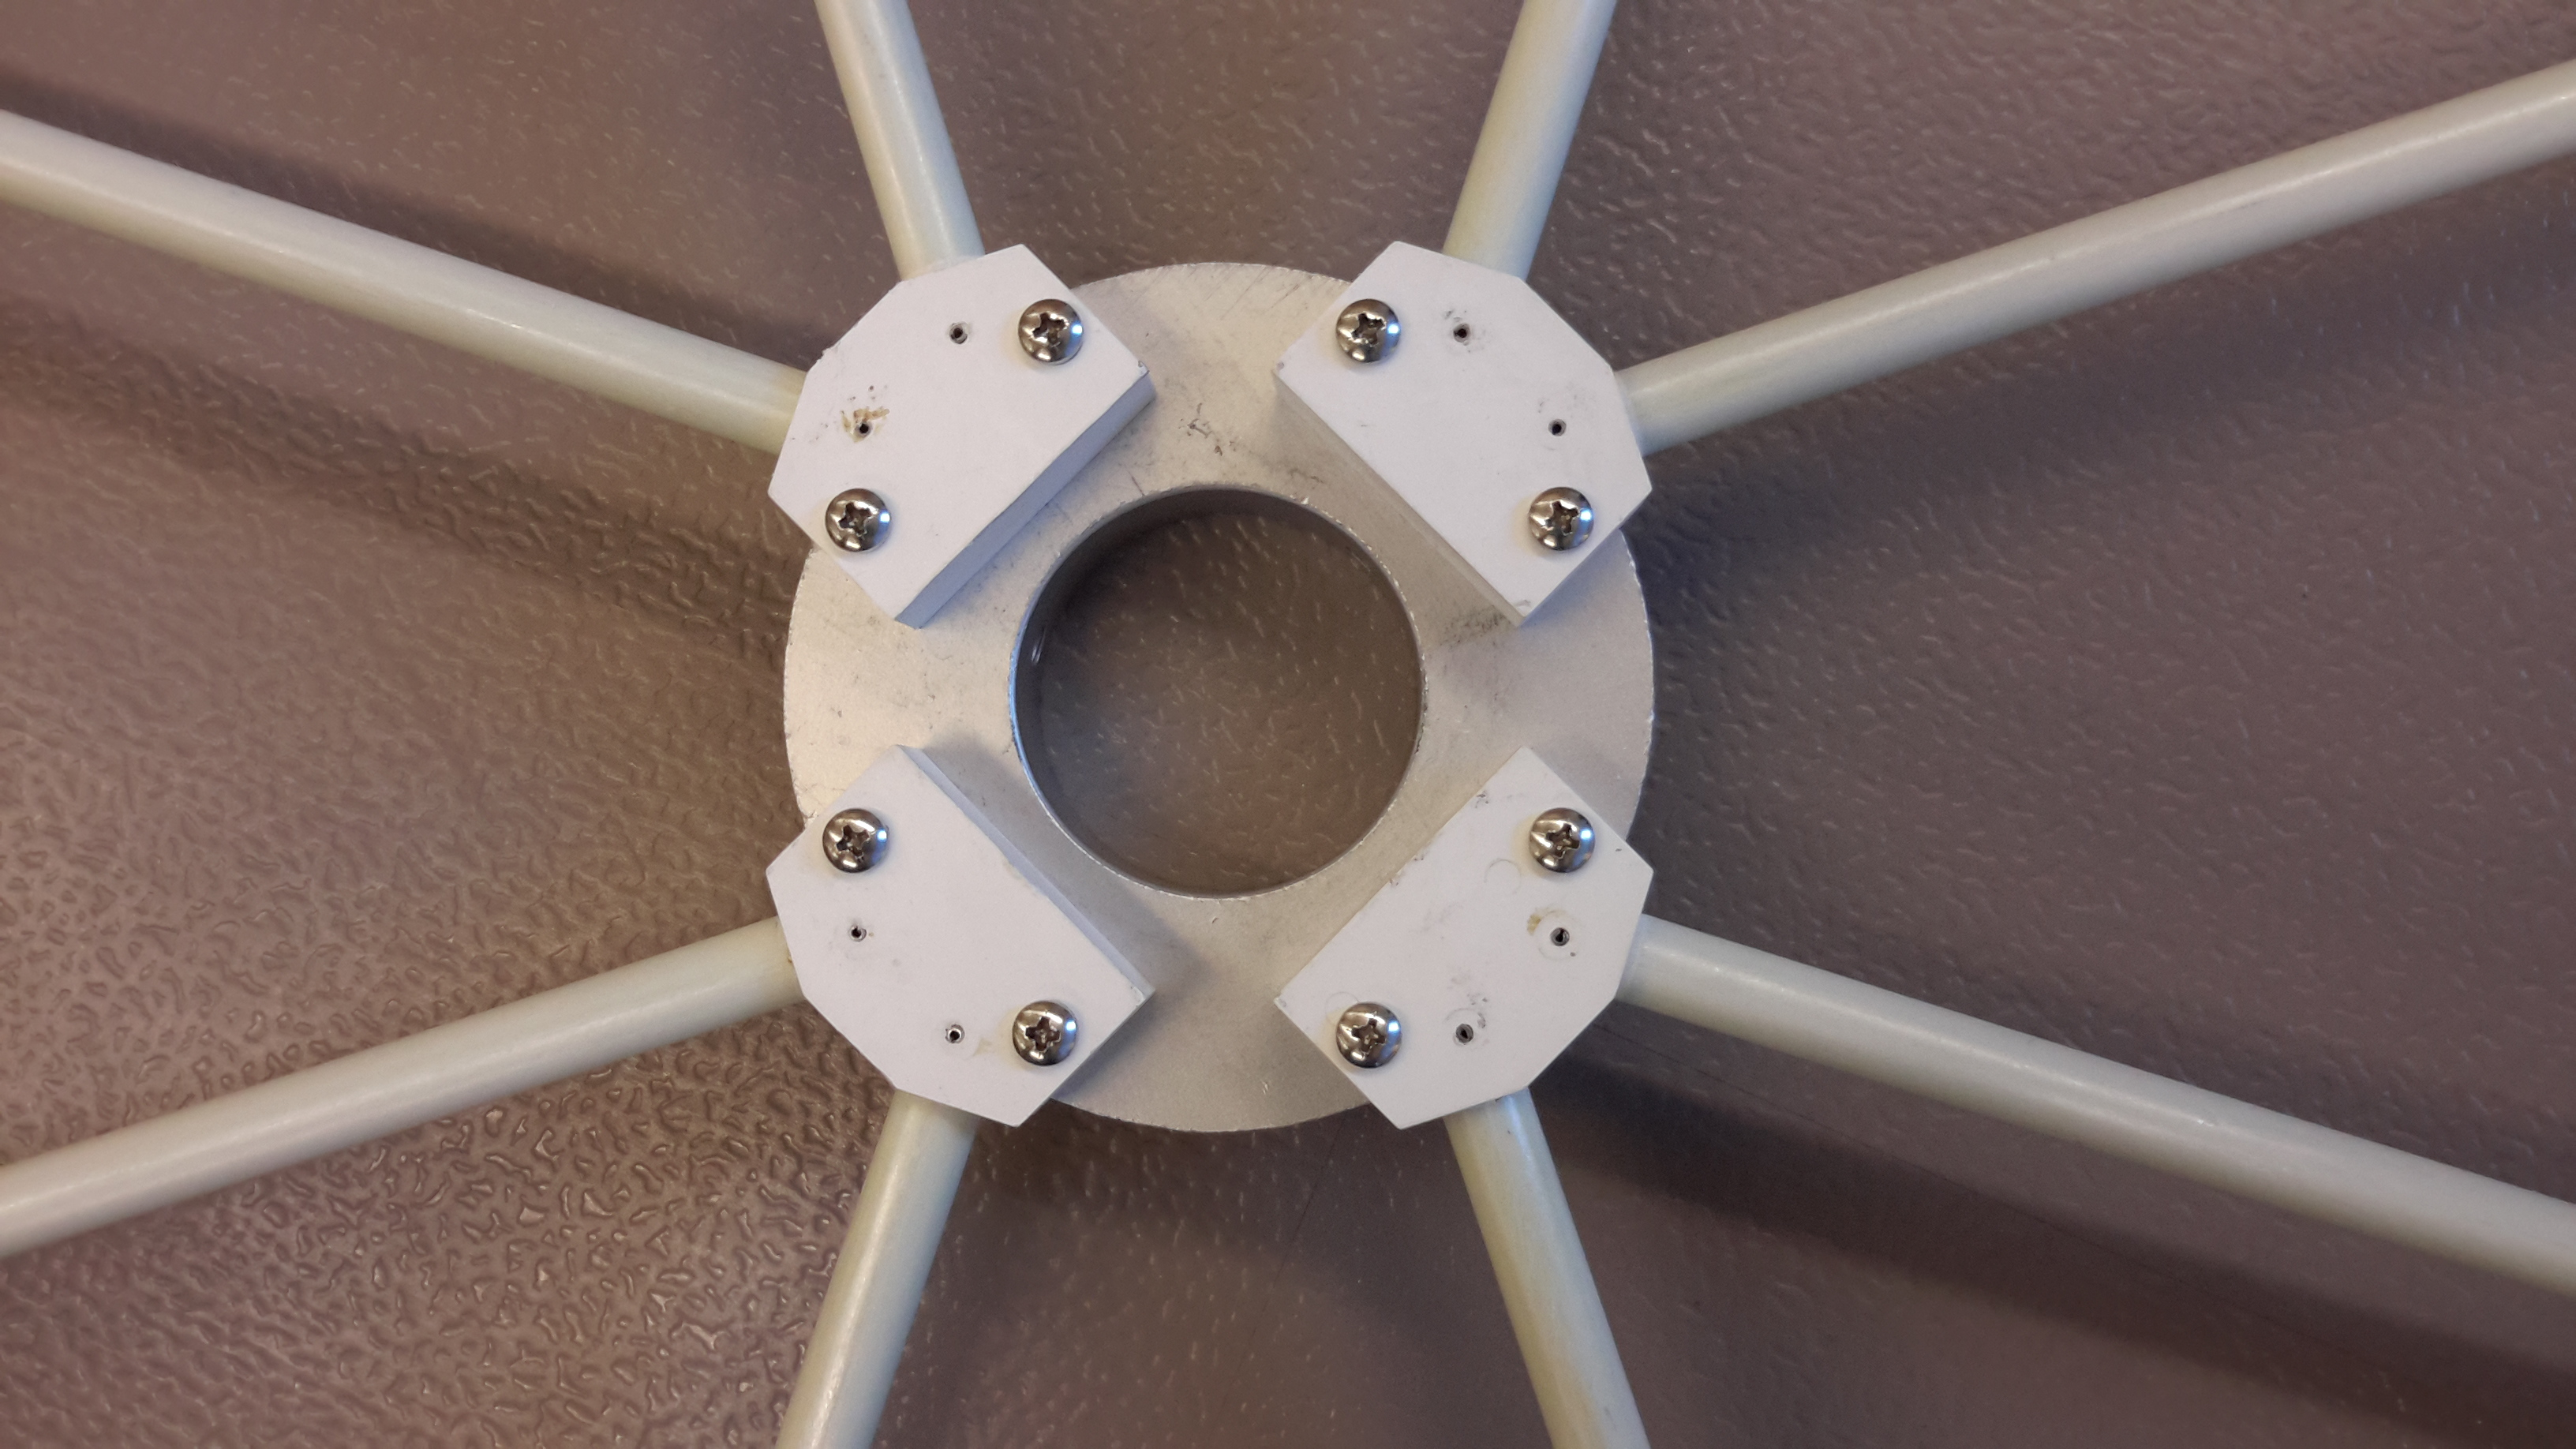
\includegraphics[width=\linewidth]{plots/20141125_100047.jpg}
      \caption{Close up of fully constructed triangle assembly. \label{TriZoom}}
\end{figure}

\newpage

\section{Mast Installation} \label{MastInstSec}
	\subsection{Required Tools}
		\begin{itemize}
			\item 2 People
			\item Post Hammer
			\item Post Level
			\item Wire cutters
		\end{itemize}
	\subsection{Required Materials}
		\begin{itemize}
			\item Mast (Part No. LWA10-102)
			\item Post Collar (Part of oz post assembly 30040)
		\end{itemize}
	\subsection{Prerequisite Tasks}
		\begin{itemize}
			\item Oz Post (Ground Stake) Installation (Not part of this document)
		\end{itemize}
	\subsection{Procedure}
		\begin{enumerate}
			\item \emph{Hammering in the post} \\ Two people are needed for this task -- one to hammer in the mast and one to monitor whether it's level throughout. When constructing several antenna elements, switching roles is recommended as the hammering is exhausting. Please wear gloves while hammering to absorb some of the impact.
			\item \emph{Clear the top of the Oz Post} \\ Remove any dirt or debris until the top of all four of the Oz Post's vanes are visible. Remove numbering stakes and/or flags and put aside, close by. If necessary, use wire cutters to remove the flag from the inside of the oz post.
			\item \emph{Place mast} \\ Slide mast into Oz Post aligned such that the slot (cut opening on the side of the mast) is near the ground and pointed towards the 1" HDPE flexible conduit emerging from the ground. Align the hole with the conduit.
			\item \emph{Collar Placement} \\ Slide collar over the top of the mast and seat it over the top of the Oz Post.
			\item \emph{Alignment $\&$ Hammering} \\ Note: The post level is magnetic and will stick to the mast. However, it will not stay on while the collar is being hammered onto the Oz Post/mast. \\ Place post level near the top of the mast and align the post vertically, checking both north/south and east/west directions. Hold the post and level in place while the second person lightly strikes the collar with the post hammer a few times, rechecking the alignment \emph{between each strike}. It might be necessary for the person checking the level to lean onto the mast to hold it in place while the collar is being hammered into place. (\emph{Be careful. The shock from the hammering can be unpleasant!}) Once the collar has been started one can hammer more vigorously while the second person still keeps an eye on the alignment, until the bottom of the collar is flush with (or close to) the top of the vanes of the Oz Post.
			\item \emph{Number stake placement} \\ As a final step, assure that the numbering stake is placed near the installed mast. The colored flag can be put in the trash or saved for another project.
		\end{enumerate}

\section{Ground Screen Placement} \label{GNDScreenPlaceSec}
	\subsection{Required Tools}
		\begin{itemize}
			\item 2 People
			\item Mini-Sledge Hammer
			\item Wire Cutters
			\item Shovel
			\item Garden Rake
		\end{itemize}
	\subsection{Required Materials}
		\begin{itemize}
			\item Ground Screen
			\item 8 stakes
			\item Alignment jig
			\item Spare Hub (optional)
		\end{itemize}
	\subsection{Prerequisite Tasks}
		\begin{itemize}
			\item Ground Screen Fabrication (See Section \ref{GNDscreenFabSec})
			\item Mast Installation (See Section \ref{MastInstSec})
		\end{itemize}
	\subsection{Procedure}
		\begin{enumerate}
			\item \emph{Level surrounding terrain} \\ Level the ground around the mast with a shovel and/or rake before installing. Enough of the area should be cleared to be able to place the whole ground screen.
			\item \emph{Cut out center of screen} \\ Note: This step can be done as part of the ground screen fabrication section (Section \ref{GNDscreenFabSec}). If already completed, skip this step. Unroll screen to be convex (i.e. the edges of the screen curve towards the ground). Locate the intersection of wires located in the middle (15 squares to every side of the screen). Using wire cutters, cut the wires flush such that there is a 4 square empty section in the center of the screen.
			\item \emph{Place screen over mast} \\ Pick up the screen and slide the mast through the enlarged center hole.
			\item \emph{Align the screen visually} \\ Rotate the screen so that the seem (where the two sections overlap) is oriented in the North-South direction. This can be done by using the alignment tool.
			\item \emph{Feed conduit through screen} \\ Identify the square positioned above where the 1" HDPE conduit emerges from the ground. Partially lift the screen and feed the conduit through this square. \emph{Avoid kinking the conduit!!!!}
			\item \emph{Stake down aligned screen} \\ Walk on the ground screen from the mast to one of the corners to flatten and stretch out the screen. Drive a stake into the corner of the screen while someone remains standing near the corner. Repeat for the remaining corners. Finally, hammer in stakes at the middle of the four sides to evenly tack down the screen. If one of the stakes is having difficulty going into the ground, it can be moved one square in either direction. As this is just used to keep the ground screen flat.
		\end{enumerate}


\section{Junction Box Assembly} \label{JuncBoxSec}
	\subsection{Required Tools}
		\begin{itemize}
			\item 1 Person
			\item Phillips Screw Driver
			\item 5/32 Allen Wrench (Long)
		\end{itemize}
	\subsection{Required Materials}
		\begin{itemize}
			\item Junction Box (Part No. LWA10-113)
			\item 10-32 UNF $\times$ $3 \over 8$ SHCS, 18-8 S.S. Bolts (Part No. LWA10-121
		\end{itemize}
	\subsection{Prerequisite Taskes}
		\begin{itemize}
			\item Ground Screen Placement (Section \ref{GNDScreenPlaceSec})
			\item Mast Installation (Section \ref{MastInstSec})
		\end{itemize}
	\subsection{Procedure}
		\begin{enumerate}
			\item \emph{Remove junction box cover} \\ Obtain one junction box for each mast and remove the two screws securing the junction box cover with a screw driver. Place the screws and cover aside.
			\item \emph{Place junction box on mast} \\ Attach the junction box onto the mast with the 10-32 UNF bolts. The junction box should be attached to the mast such that the circular opening of the junction box is facing down. Ensure all four bolts are in place and secure by using the allen wrench with an extension.
			\item \emph{Replace cover} \\ Replace the screws and cover on the attached junction box. \emph{The plastic is soft so care must be taken to not strip the material.} Do \emph{not} use an electric screwdriver during this step.
		\end{enumerate}
			

\section{Hub Installation} \label{HubInstSec}
	\subsection{Required Tools}
		\begin{itemize}
			\item Slotted Screw Driver
			\item Hub Alignment Jig
			\item Phillips Screw Driver
		\end{itemize}
	\subsection{Required Materials}
		\begin{itemize}
			\item Hub Base (Part No. LWA10-100)
			\item Hub Cover (Part No. LWA10-101)
			\item Size 12 Hose Clamp
			\item 10-14 $\times$ 1/2 Long S.S. Plastite Screws (Part No. LWA10-111)
		\end{itemize}
	\subsection{Prerequisite Tasks}
		\begin{itemize}
			\item Mast Installation (Section \ref{MastInstSec})
			\item Ground Screen Placement (Section \ref{GNDScreenPlaceSec})
			\item Junction Box Installation (Section \ref{JuncBoxSec})
			\item Triangle Assembly (Section \ref{TriAssemSec})
		\end{itemize}
	\subsection{Procedure}
		\begin{enumerate}
			\item \emph{Place triangle assembly on mast} \\ Slide the center flange part of the triangle assembly onto the mast such that the flat part of the flange is on the top, and rest it on the junction box (See Figure \ref{TriZoom} and note that the flat side is facing up in this image) . Make sure the extended part of the center flange is down so the triangles are pointing up (Figure \ref{TriComplete}) (i.e. the extended side should be resting on the junction box).
			\item \emph{Place clamp on Hub} \\ Place the hose clamp on the bottom of the hub and tighten it just enough to secure it into place. See Figure \ref{ClampedHub}.

\begin{figure}[!h]
	\center
	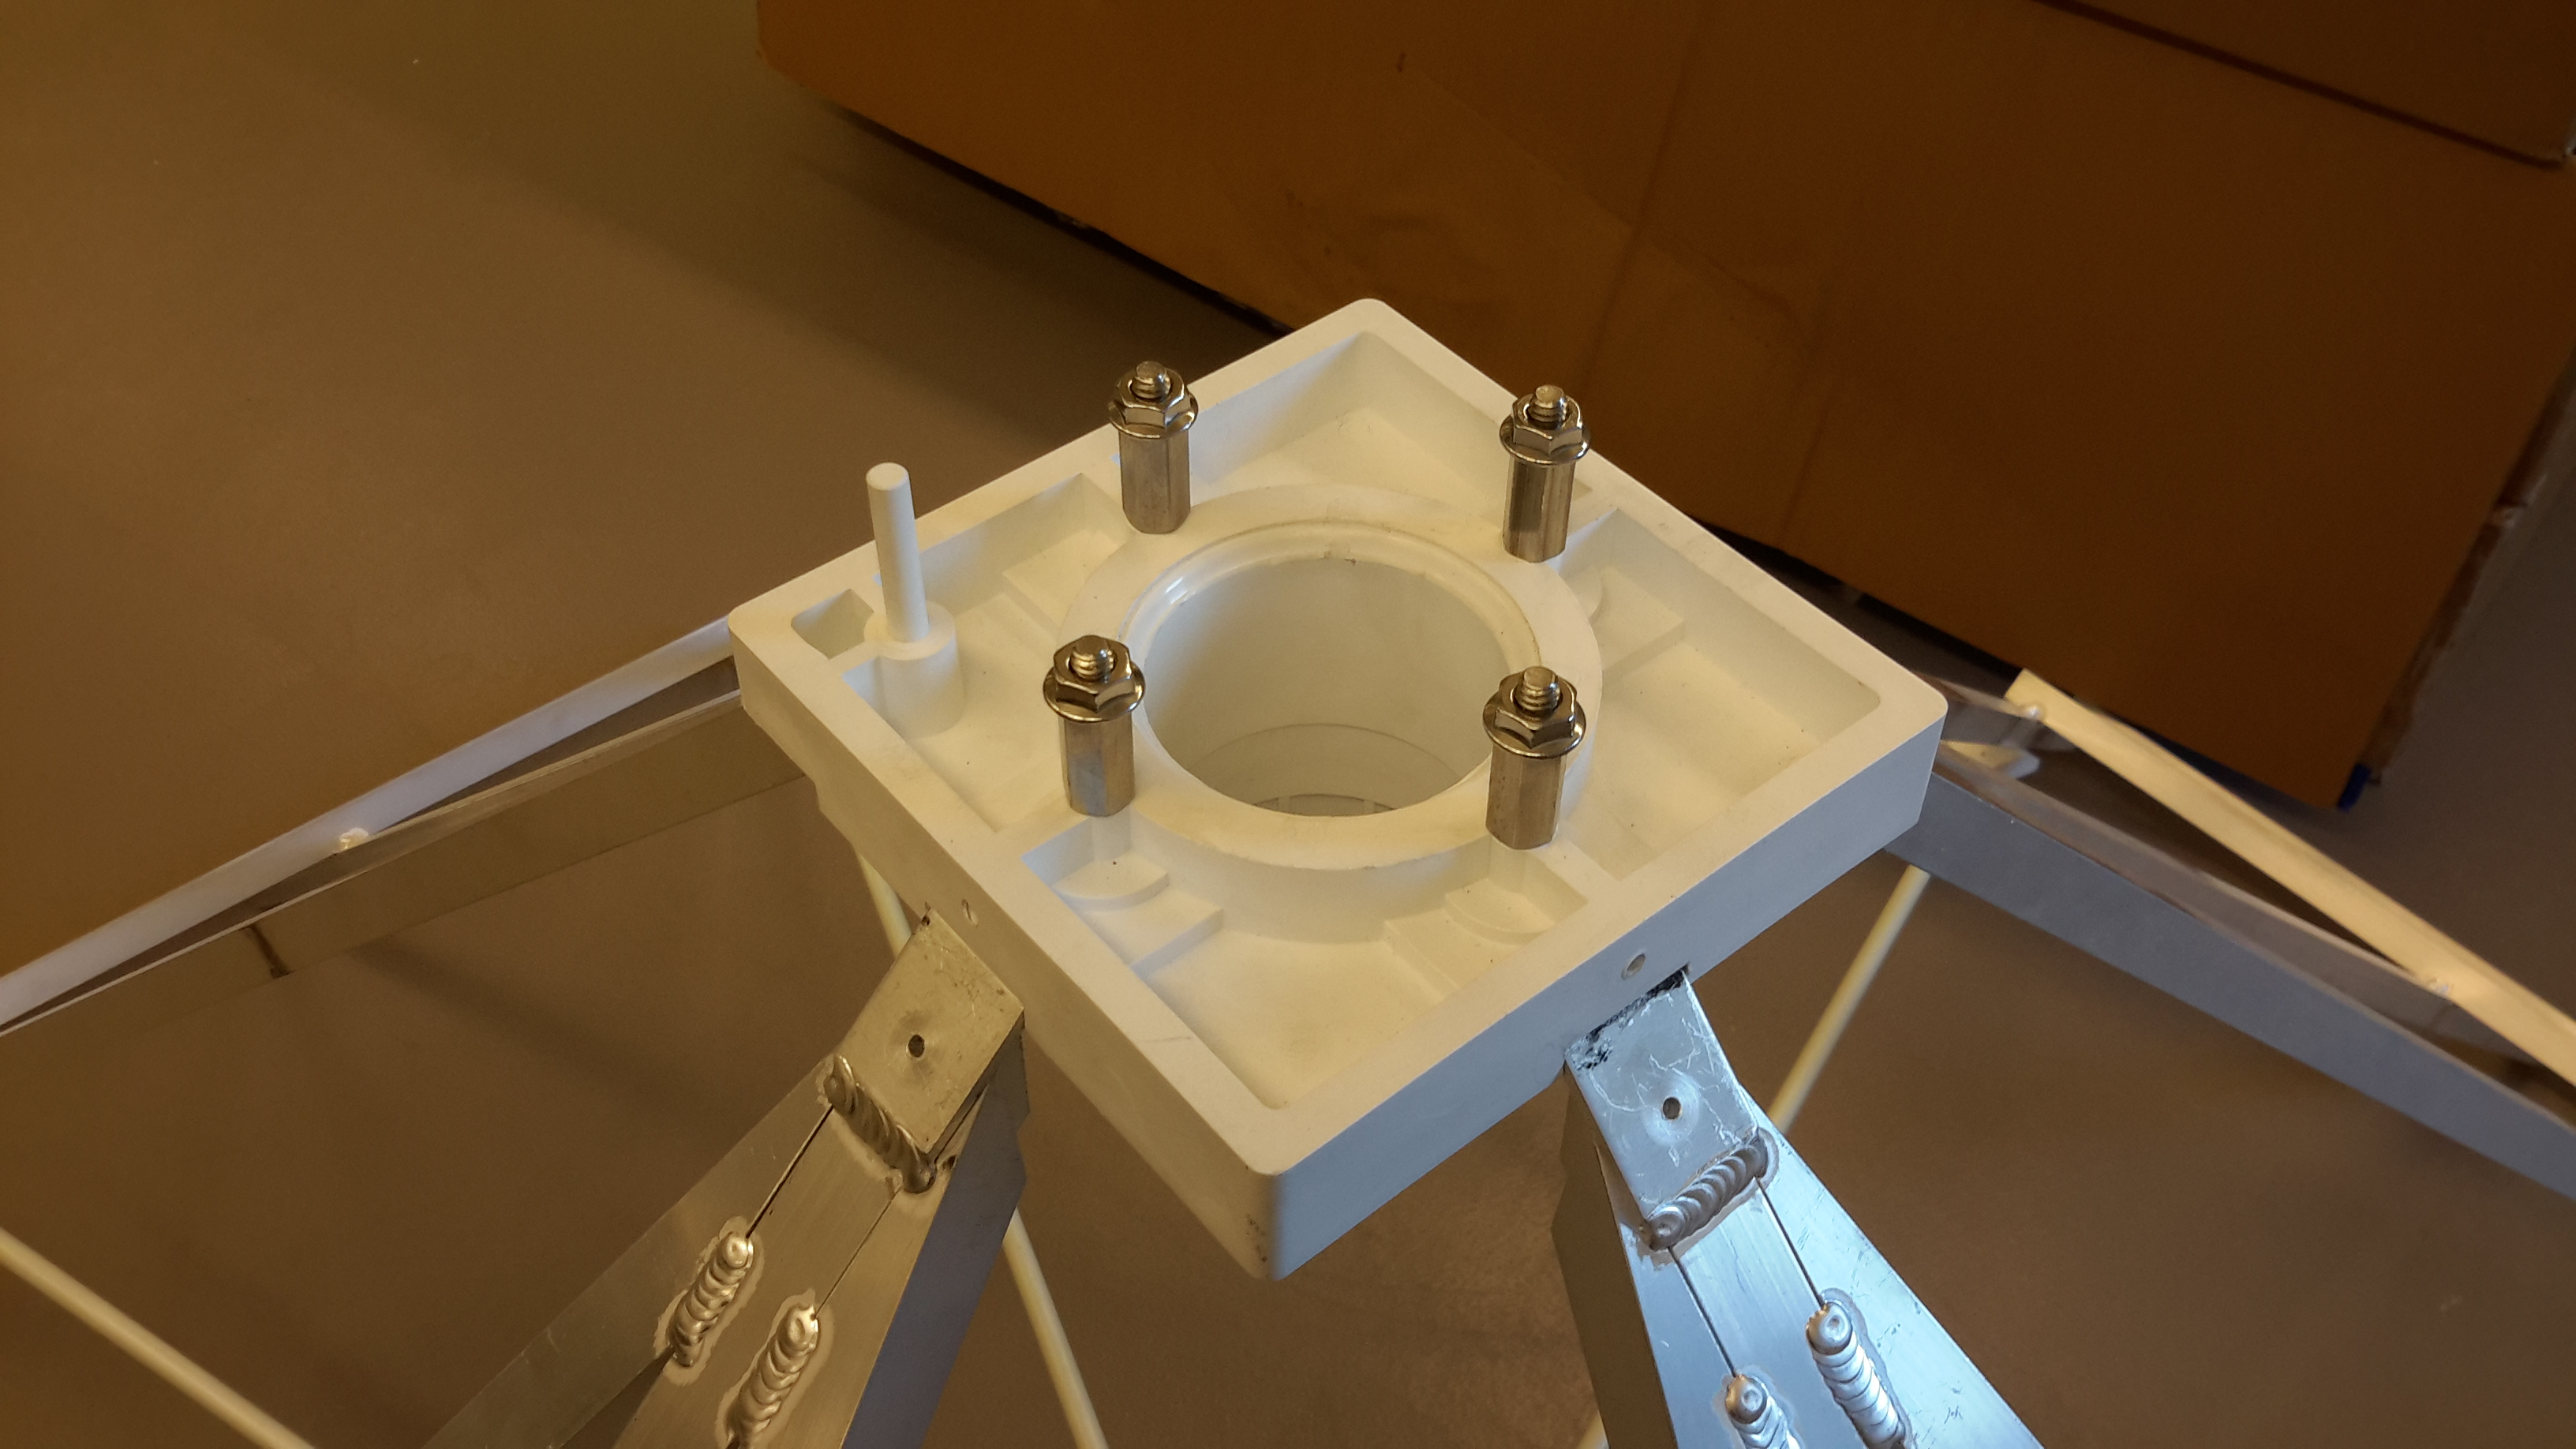
\includegraphics[width=\linewidth]{plots/20141125_112425.jpg}
	\caption{Hub without cover or FEE \label{HubCompleteSansCover}}
\end{figure}

\begin{figure}
	\center
	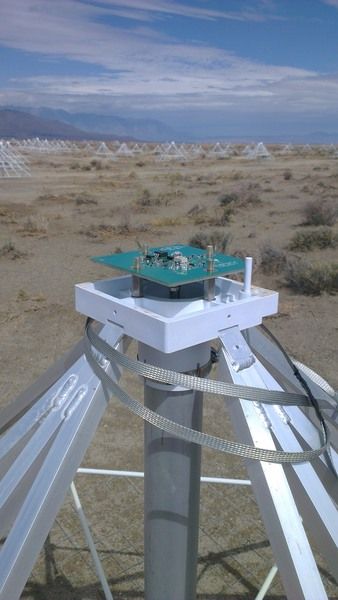
\includegraphics[width=0.7\linewidth]{plots/IMAG0068.jpg}
	\caption{Assembled hub with FEE. Hose clamp is around bottom of hub and is tightened just enough to secure it into place (Source: https://www.ocf.berkeley.edu/~rsd/ral/lwa/construction/). \label{ClampedHub}}
\end{figure}

			\item \emph{Place hub on mast} \\ Slide the hub onto the top of the mast and remove its cover. See Figure \ref{HubCompleteSansCover}.
			\item \emph{Align hub} \\ Place the alignment jig onto the stand-offs that are on the top of the hub base. Rotate the hub until the vertical cross-hairs of the alignment scope are superimposed over the point of interest.
			\item \emph{Tighten the clamp} \\ Tighten up the hose clamp that is on the base of the hub and re-check with alignment tool.
			\item \emph{Replace hub cover} \\ Remove alignment jig and place cover back onto hub. Put in at least one of the screws into the hub cover to hold the cover in place. 
			
	\end{enumerate}

\section{Final Stand Assembly}
	\subsection{Required Tools}
		\begin{itemize}
			\item 7/16 Socket Wrench with Extender
			\item 5/16 Socket Wrench
			\item 5/32 Allen wrench
		\end{itemize}
	\subsection{Required Materials}
		\begin{itemize}
			\item (4) Elements
			\item (4) $1 \over 4$ - 20 Hex Flange Nuts, 18-8 S.S (Part No. LWA10-132)
			\item (8) 10-32 UNF X 1.25 hex SEM SCREW, 18-8 S.S. (Part No. LWA10-130)
		\end{itemize}
	\subsection{Prerequisite Tasks}
		\begin{itemize}
			\item Hub Alignment and Installation (Section \ref{HubInstSec})
		\end{itemize}
	\subsection{Procedure}
		\begin{enumerate}
			\item \emph{Connect element to hub} \\ Remove the cover to the hub and set aside so it is not in the way. Put the stud that is on the underside of the hub through the tab on the element and secure in place with a flange nut (See Figure \ref{UnderHub}). This can be done by having one person hold the element in place while the other secures the nut with a socket wrench. It is easiest if the bolt is first hand tightened and then tightened with a socket wrench. Use \emph{great care} not to over tighten at this point.
			
\begin{figure}[!h]
	\center
	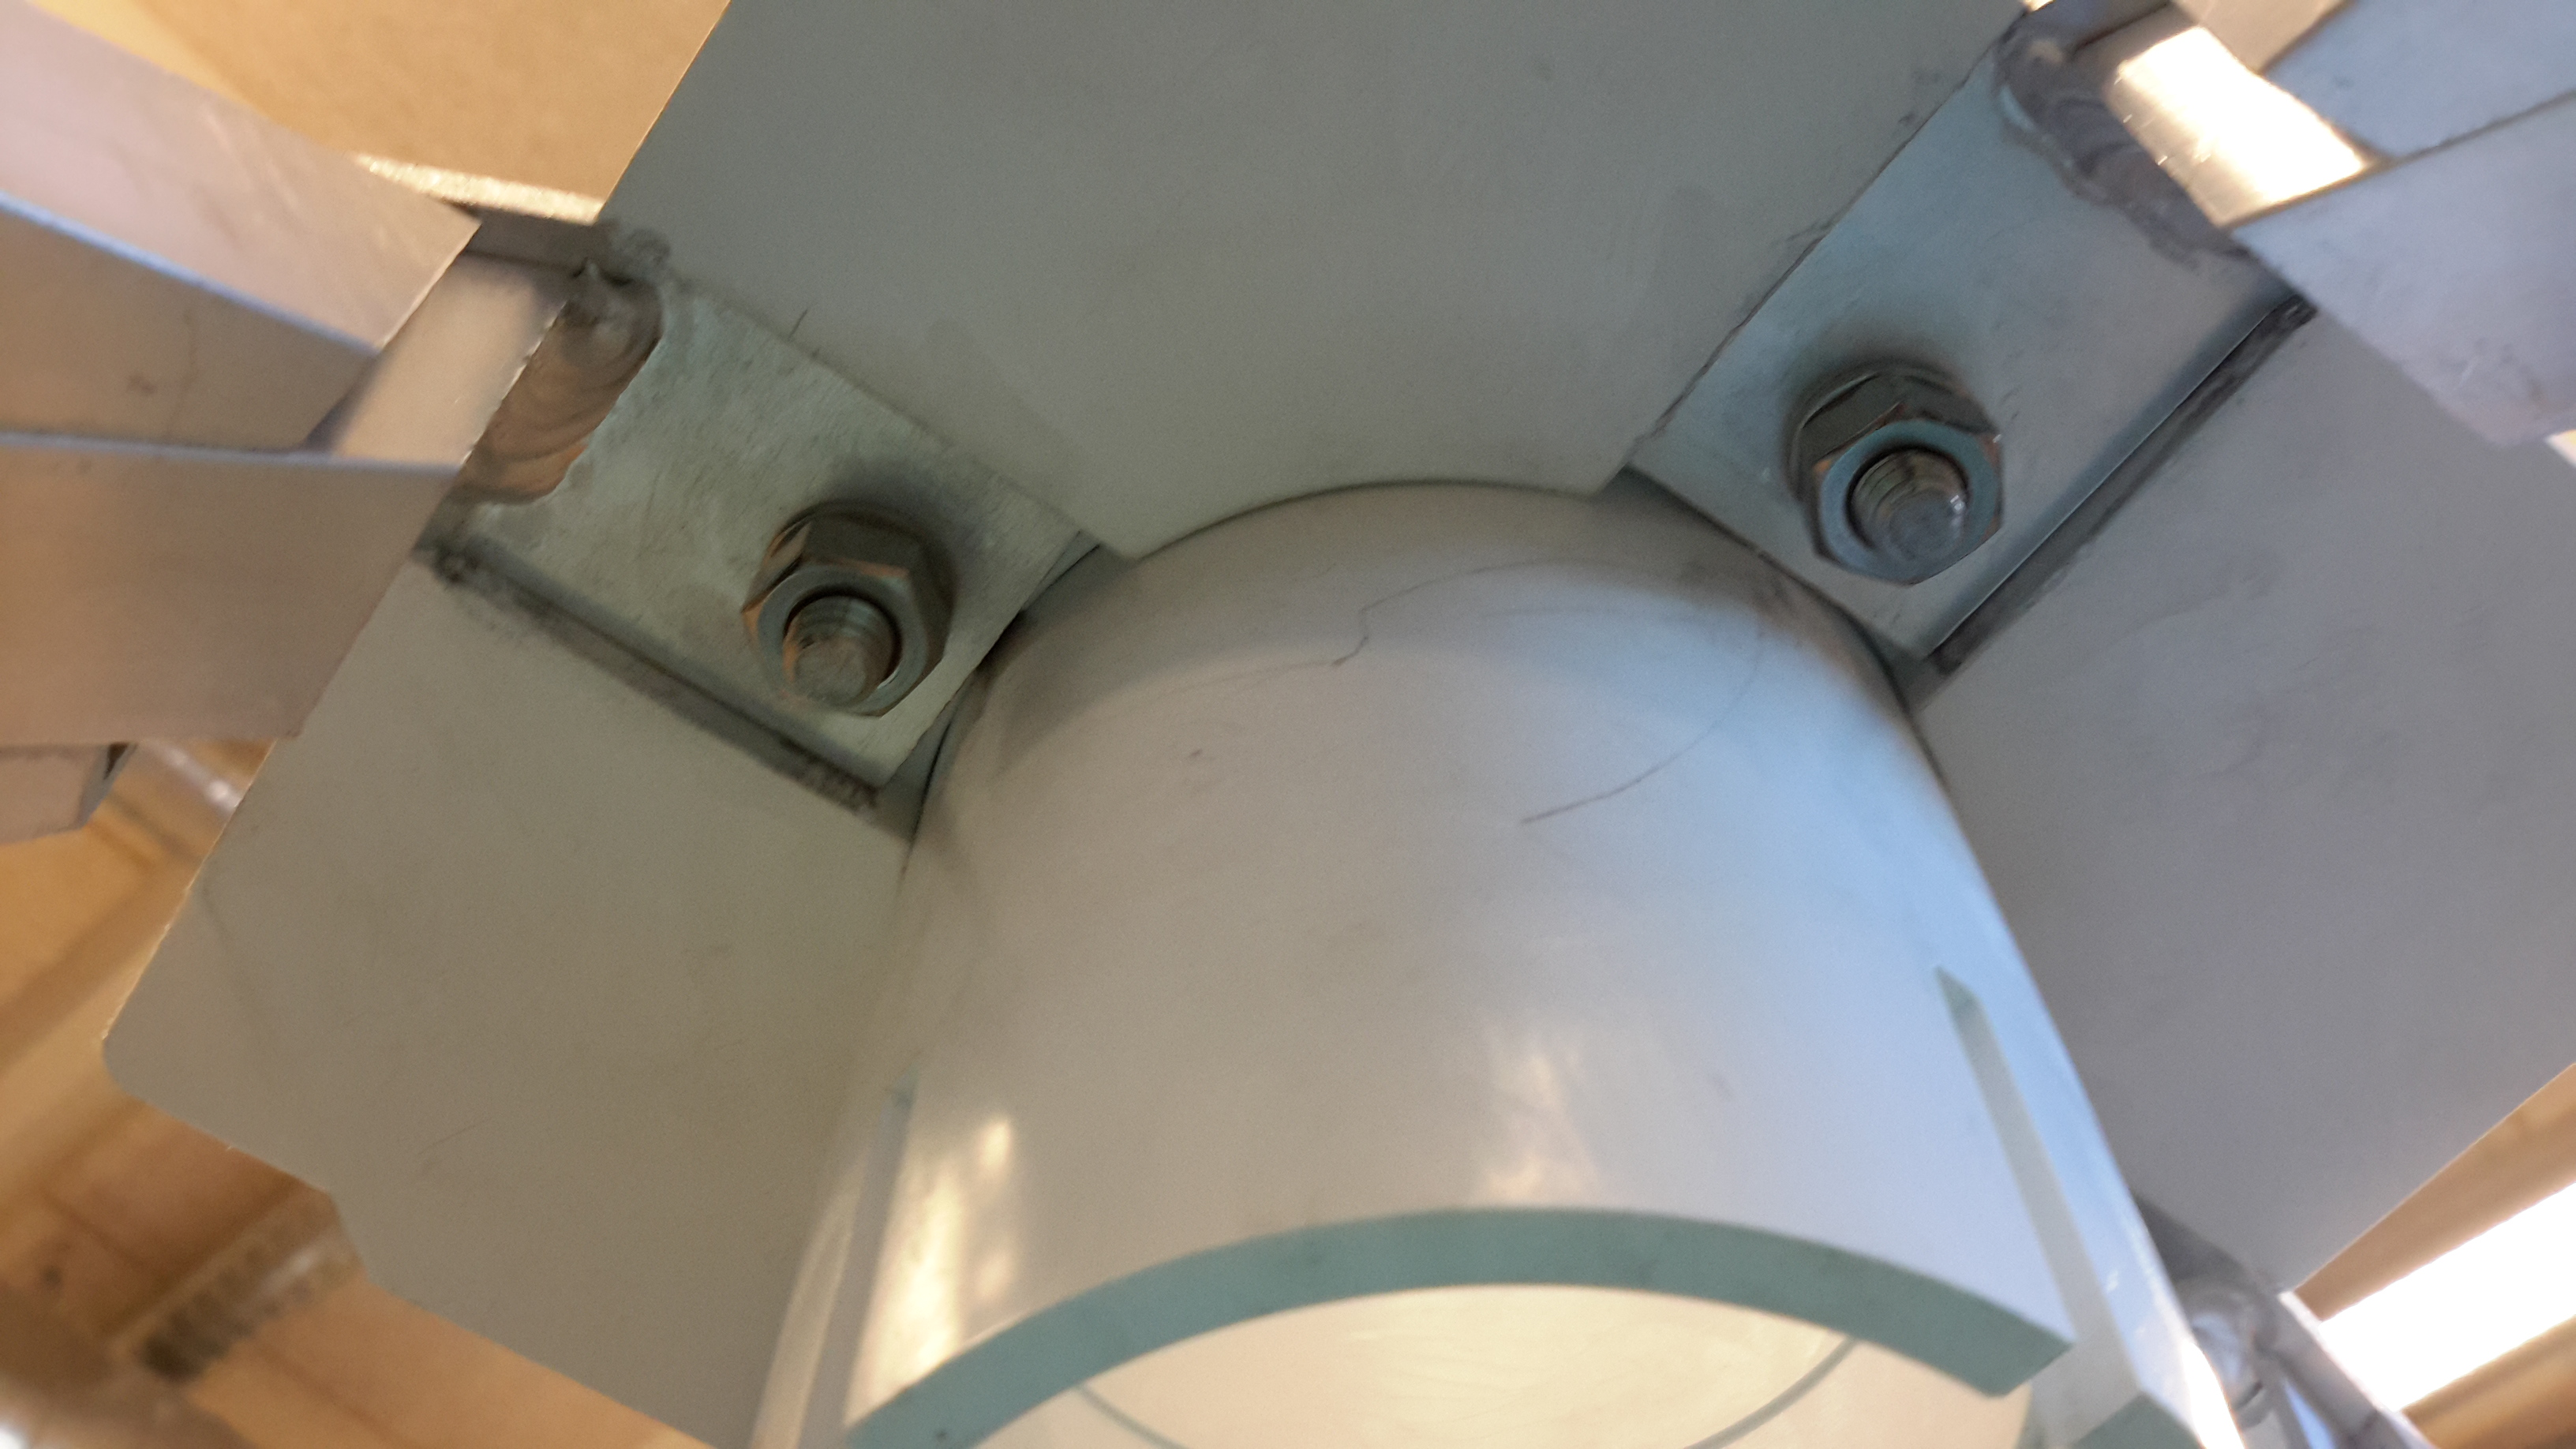
\includegraphics[width=\linewidth]{plots/20141125_110653.jpg}
	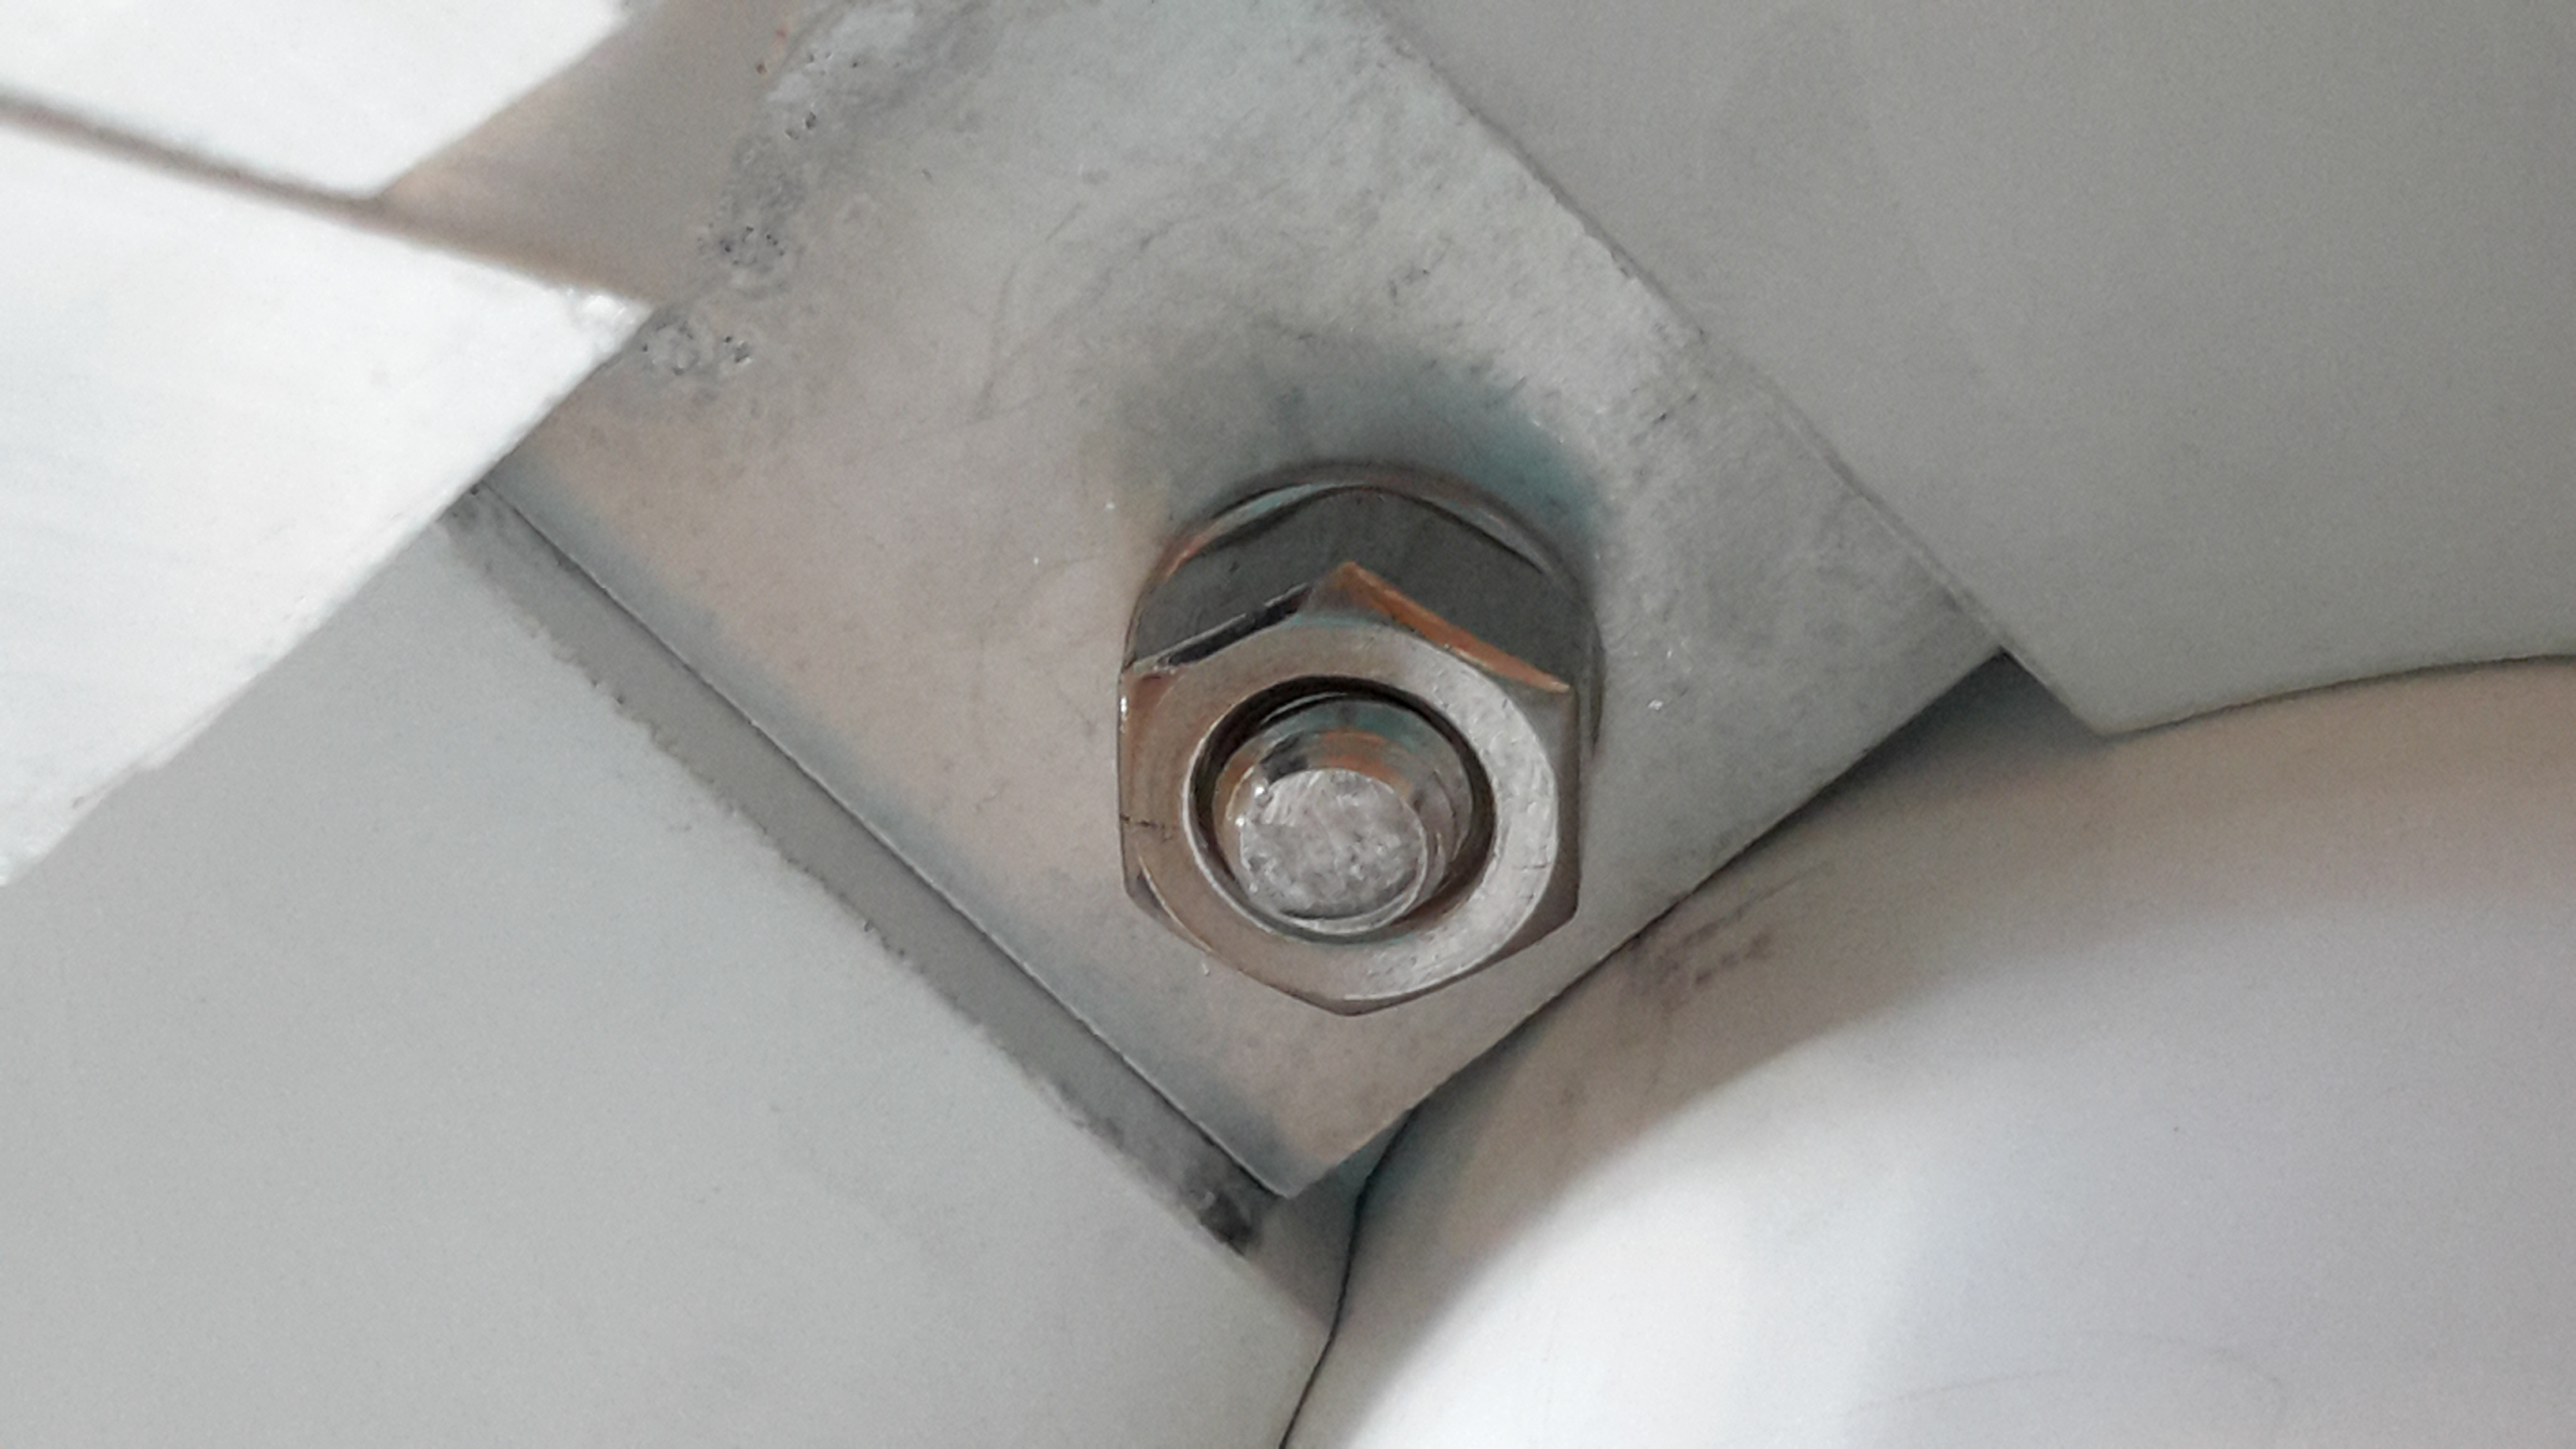
\includegraphics[width=\linewidth]{plots/20141212_153321.jpg}
	\caption{Top: The underside of the hub with flange nuts in place. Bottom: Close up of element tab attached to underside of hub. \label{UnderHub}}
\end{figure}	

			\item \emph{Attach element to triangle assembly} \\ Slide the triangle assembly along the mast until its level with the bolt holes in the element. Secure element to the triangles so that it spans the gap between two triangles, using two bolts. Do not fully tighten these bolts. You want the elements to retain some freedom of movement at this point. If fully tightened before all elements are attached, the remaining elements will be very difficult to attach. See Figure \ref{Tri+Element}.

\begin{figure}[!p]
	\center
	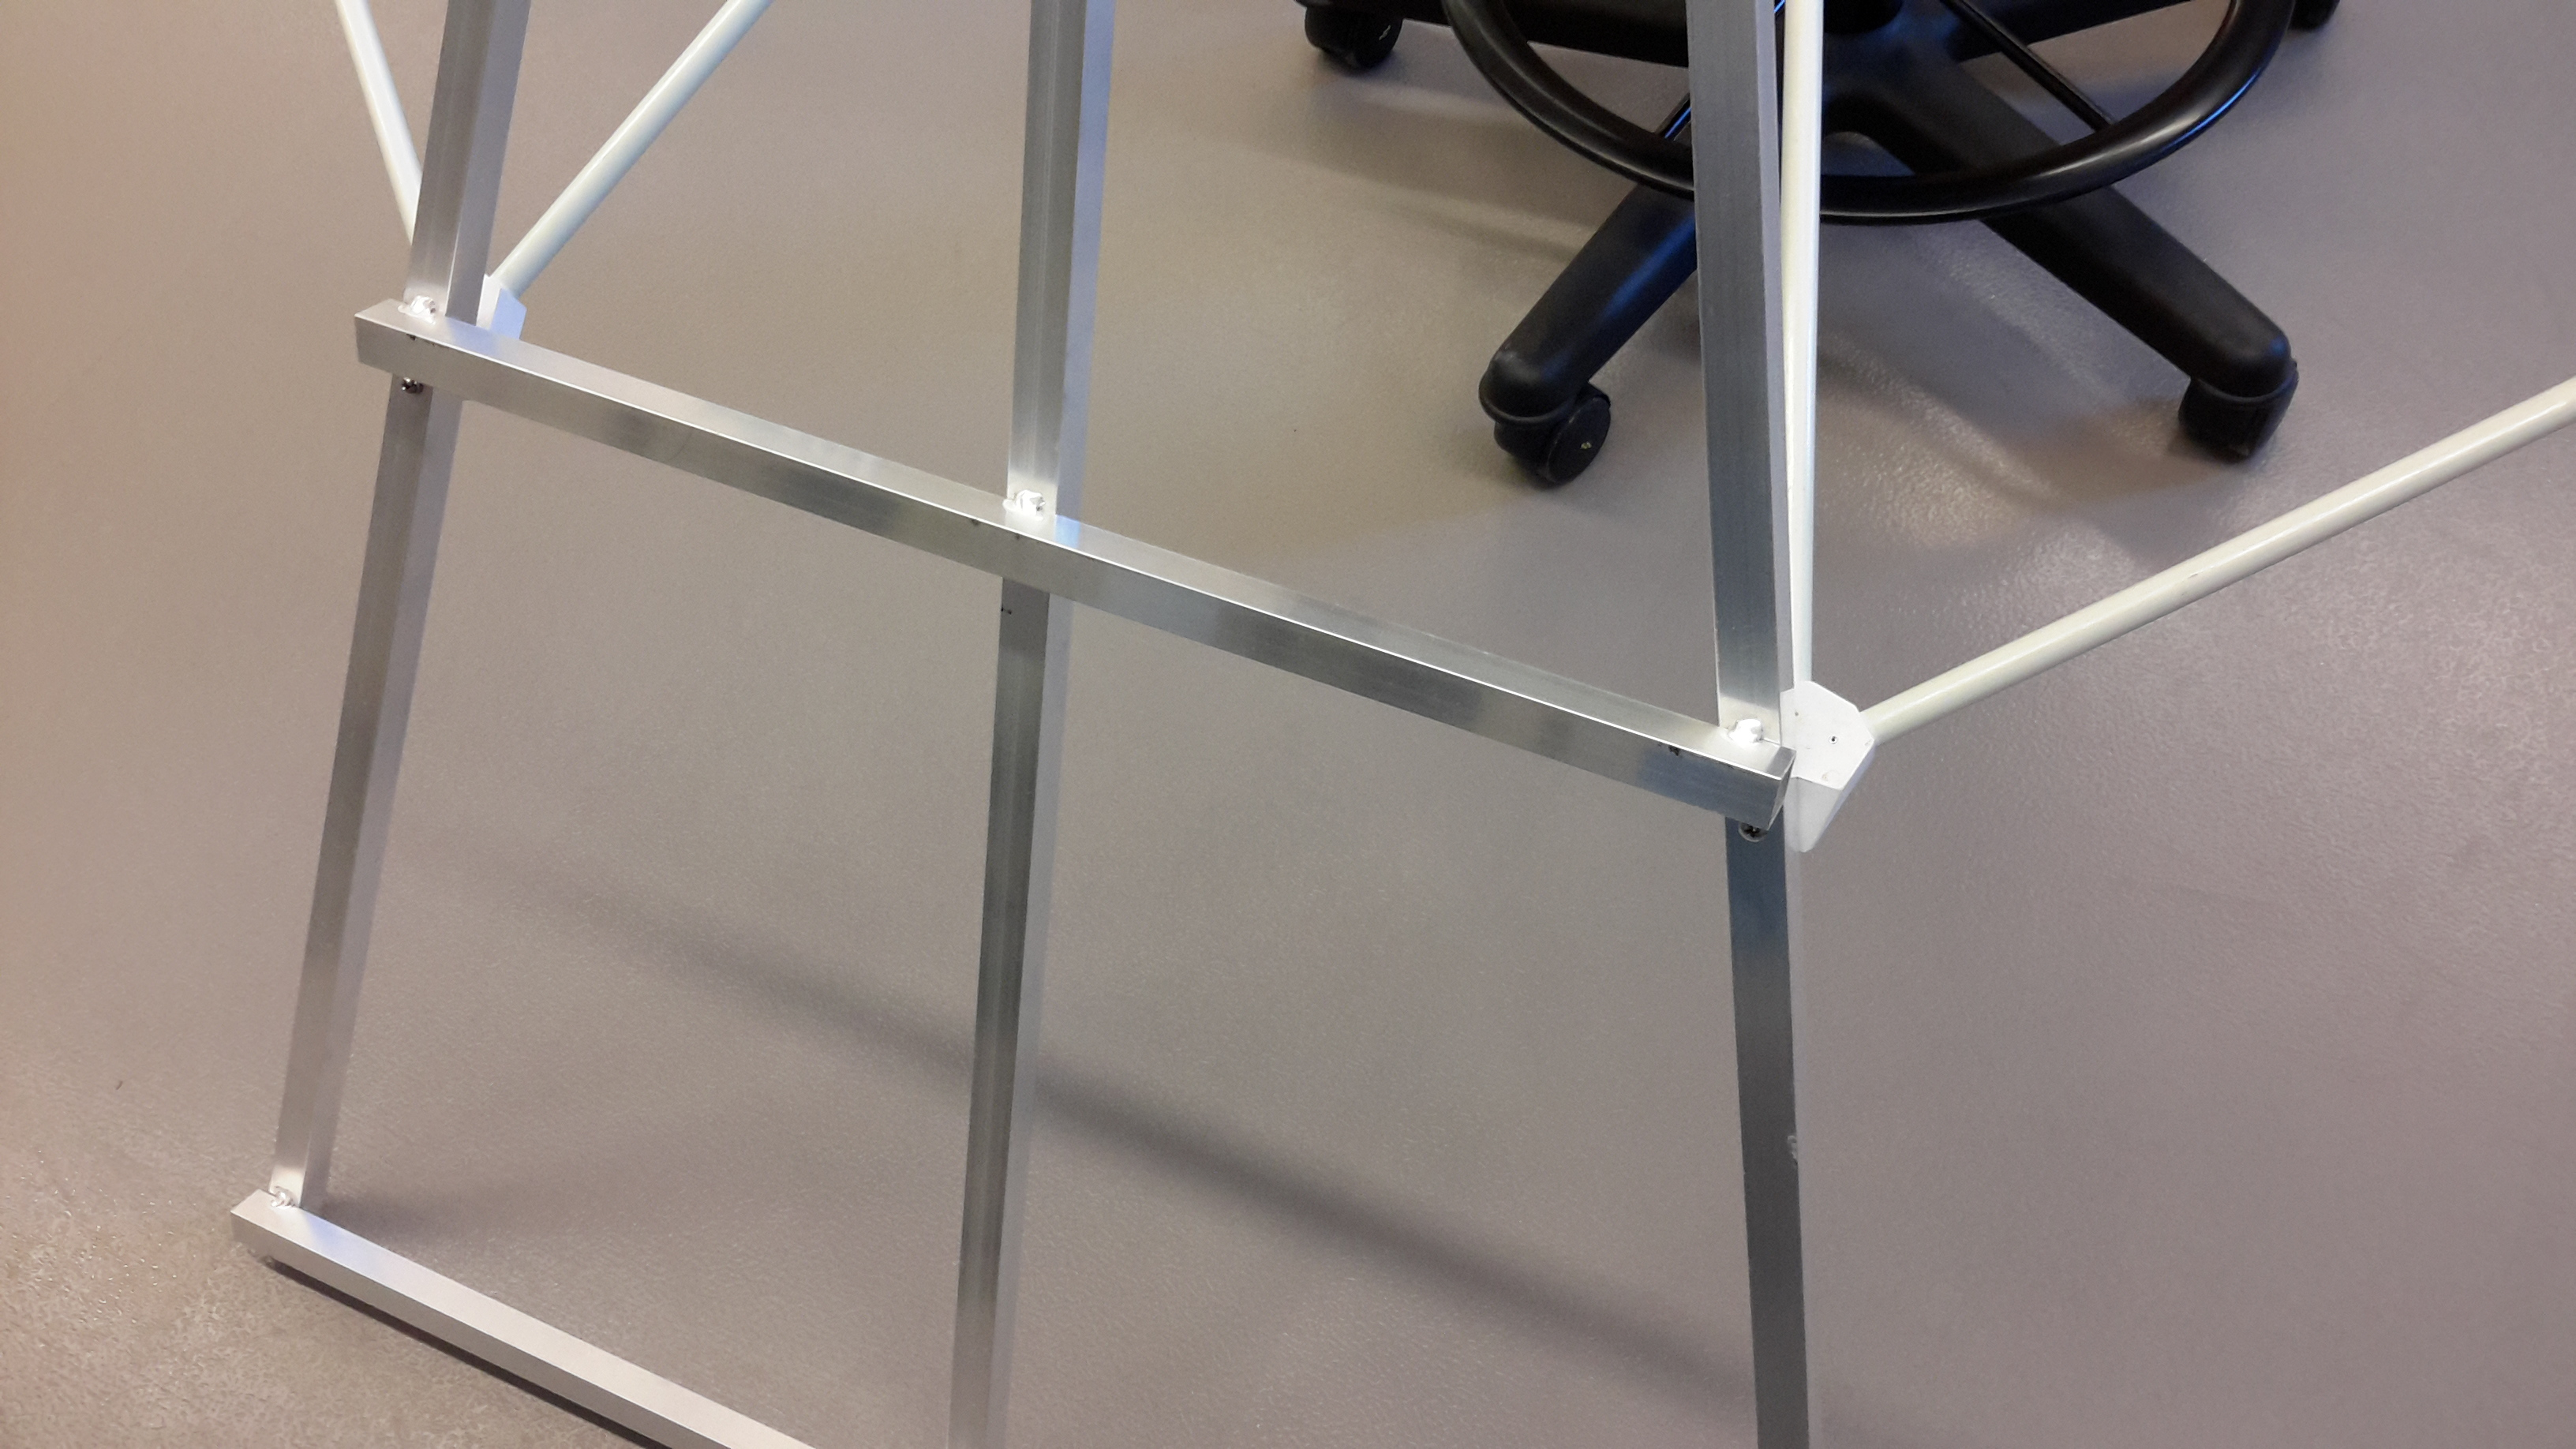
\includegraphics[width=0.7\linewidth]{plots/20141125_102636.jpg}
	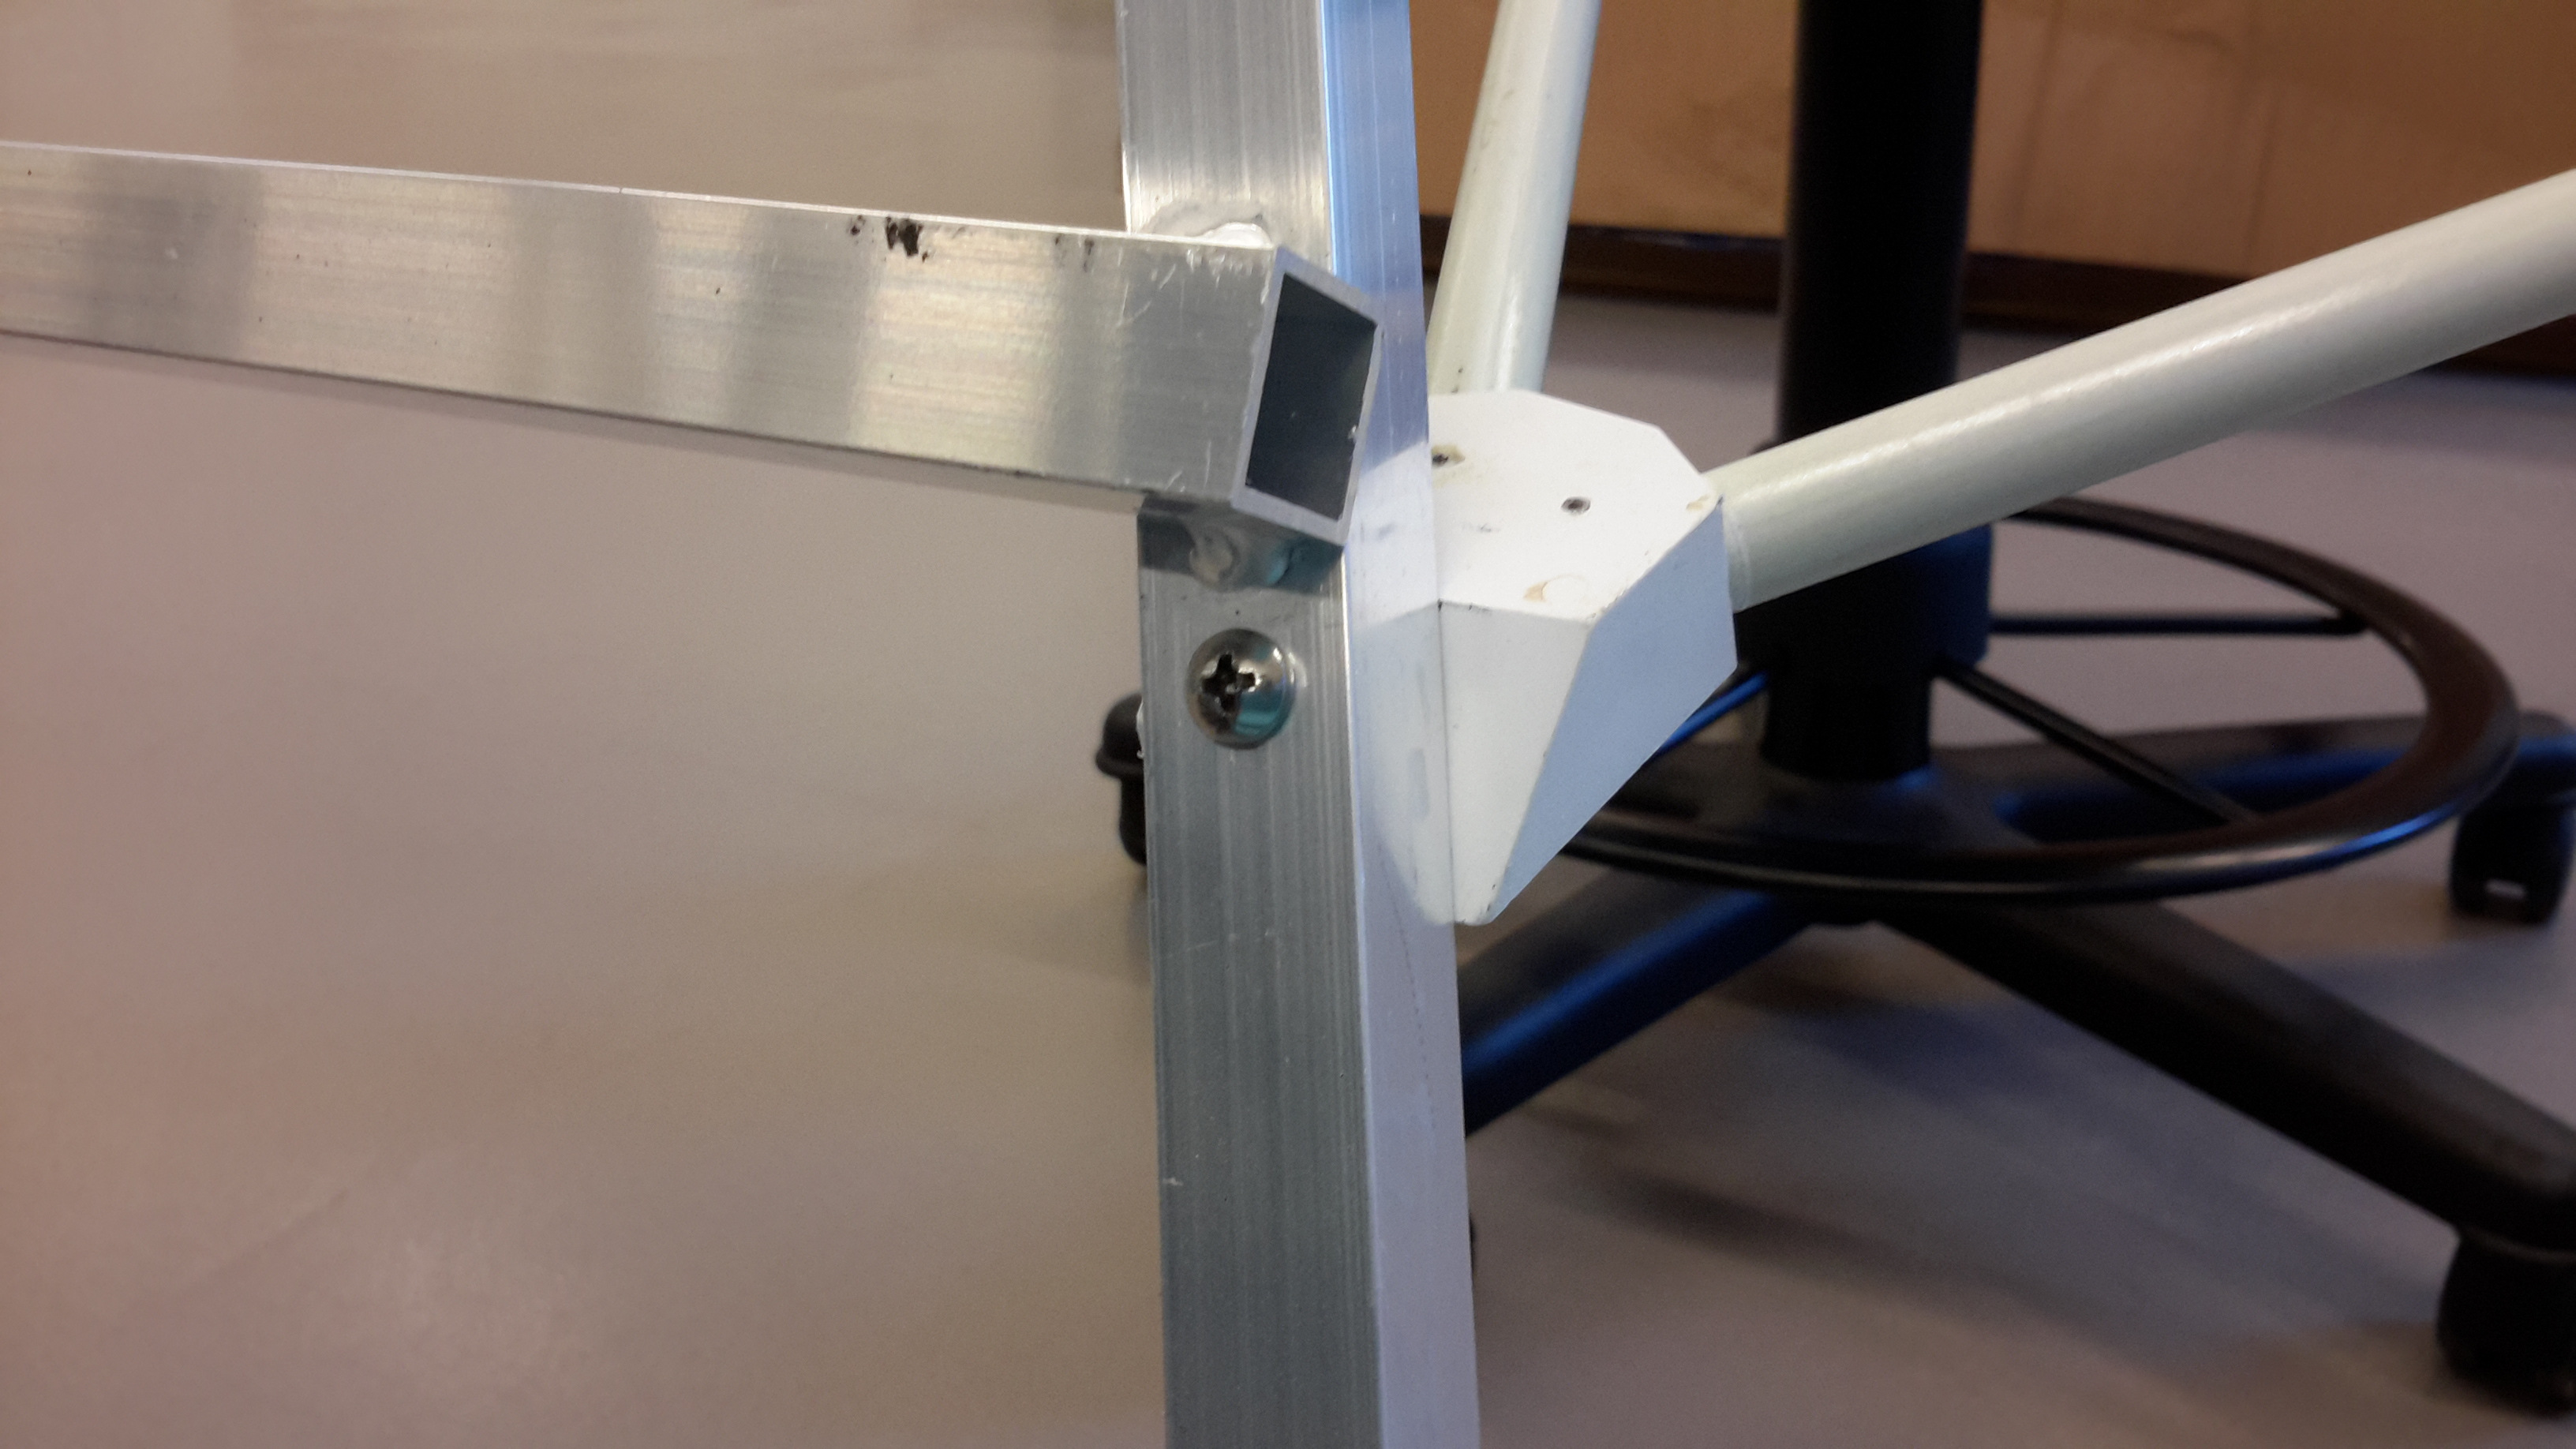
\includegraphics[width=0.7\linewidth]{plots/20141125_102607.jpg}
	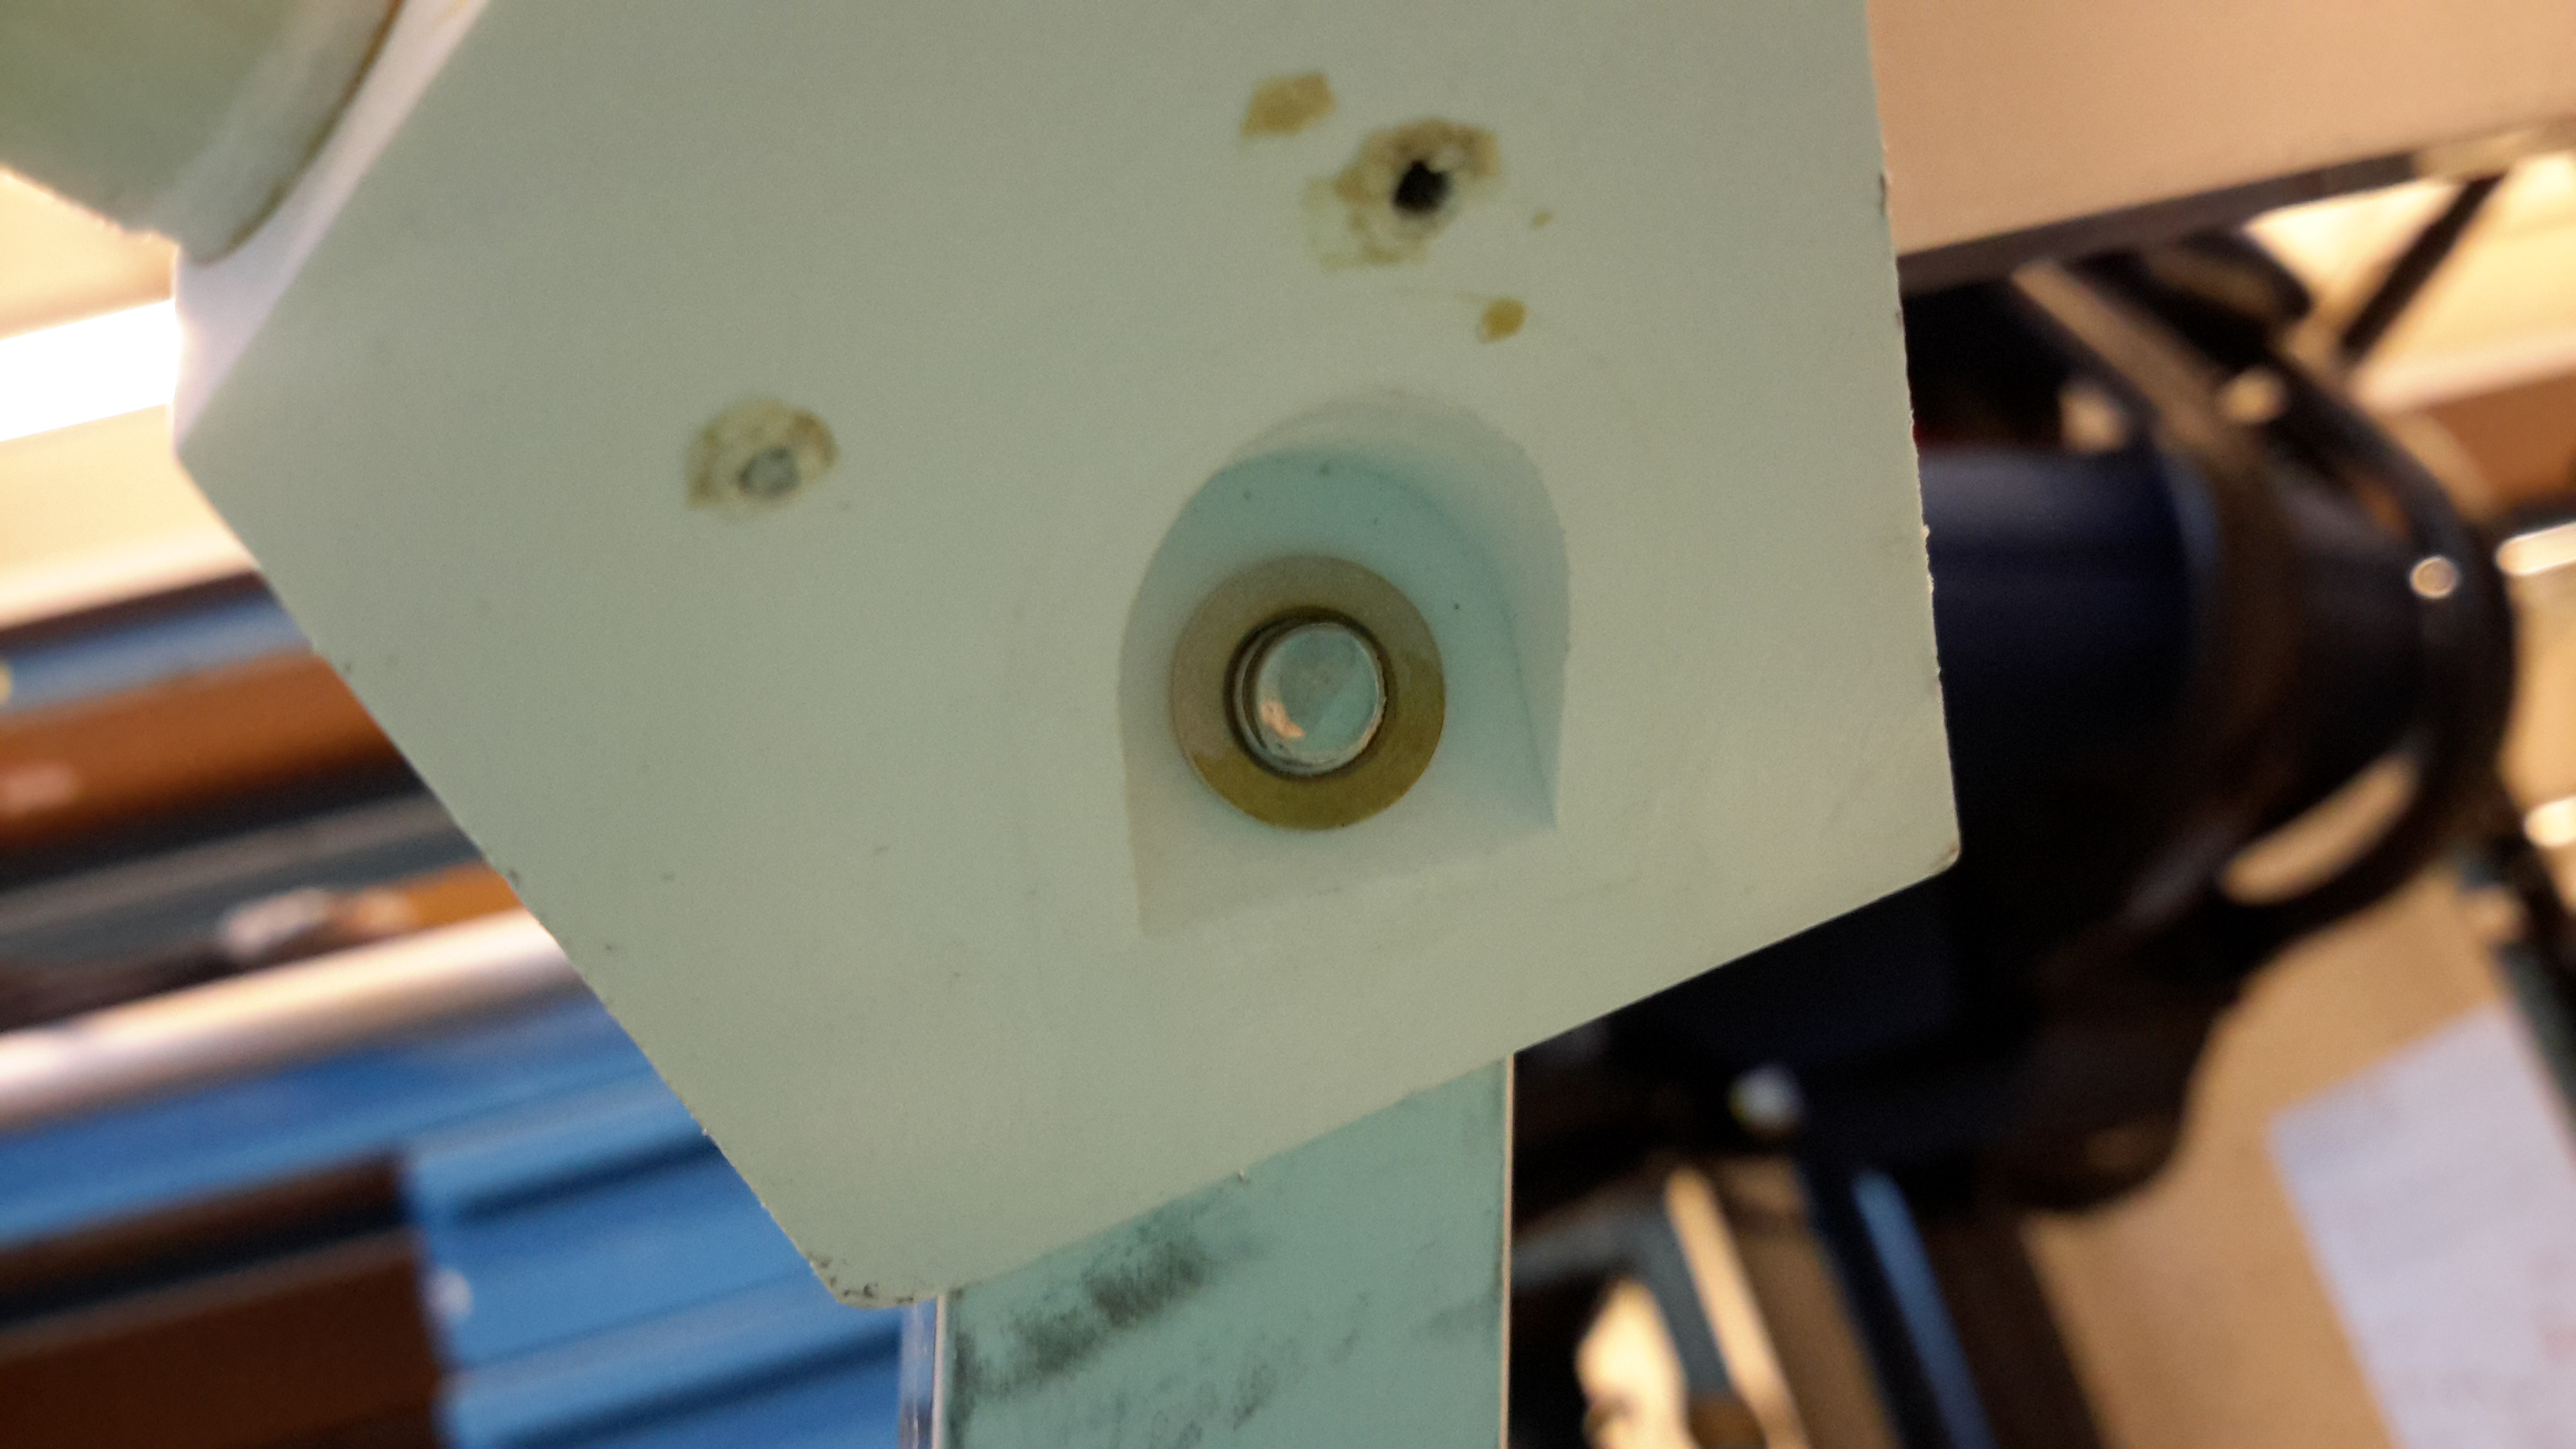
\includegraphics[width=0.7\linewidth]{plots/20141125_102622.jpg}
	\caption{Top:  Attach the element to the triangle with the SEM screws. Middle: Make sure slanted edge of triangle is facing upward to attach to element. Bottom: Underside of triangle corner attached to element. \label{Tri+Element}}
\end{figure}
	
			\item \emph{Attach opposing element} \\ Repeat steps 1 and 2 to attach an element on the opposite side of the stand. Again, do not fully tighten the bolts.
			\item \emph{Attach remaining elements} \\ Repeat steps 1 and 2 until all four elements are in place.
			\item \emph{Fully tighten bolts} \\ Once all the elements have been loosely fit onto the stand, go back and fully tighten the bolts. Be sure to double check that all elements have been secured.
			\item \emph{Secure flange to mast} \\ Finally, slide the flange up the mast a bit to relieve the strain on the triangle assembly, until the arms of the triangles are level with the ground, and tighten the set screws with an allen wrench to secure the flange to the mast. See Figure \ref{AlmostCompleteElement} for the (nearly) fully assembled element (missing mast, junction box, and ground stake/ground screen due to being assembled in the lab for testing).
	\end{enumerate}

\begin{figure}
	\center
	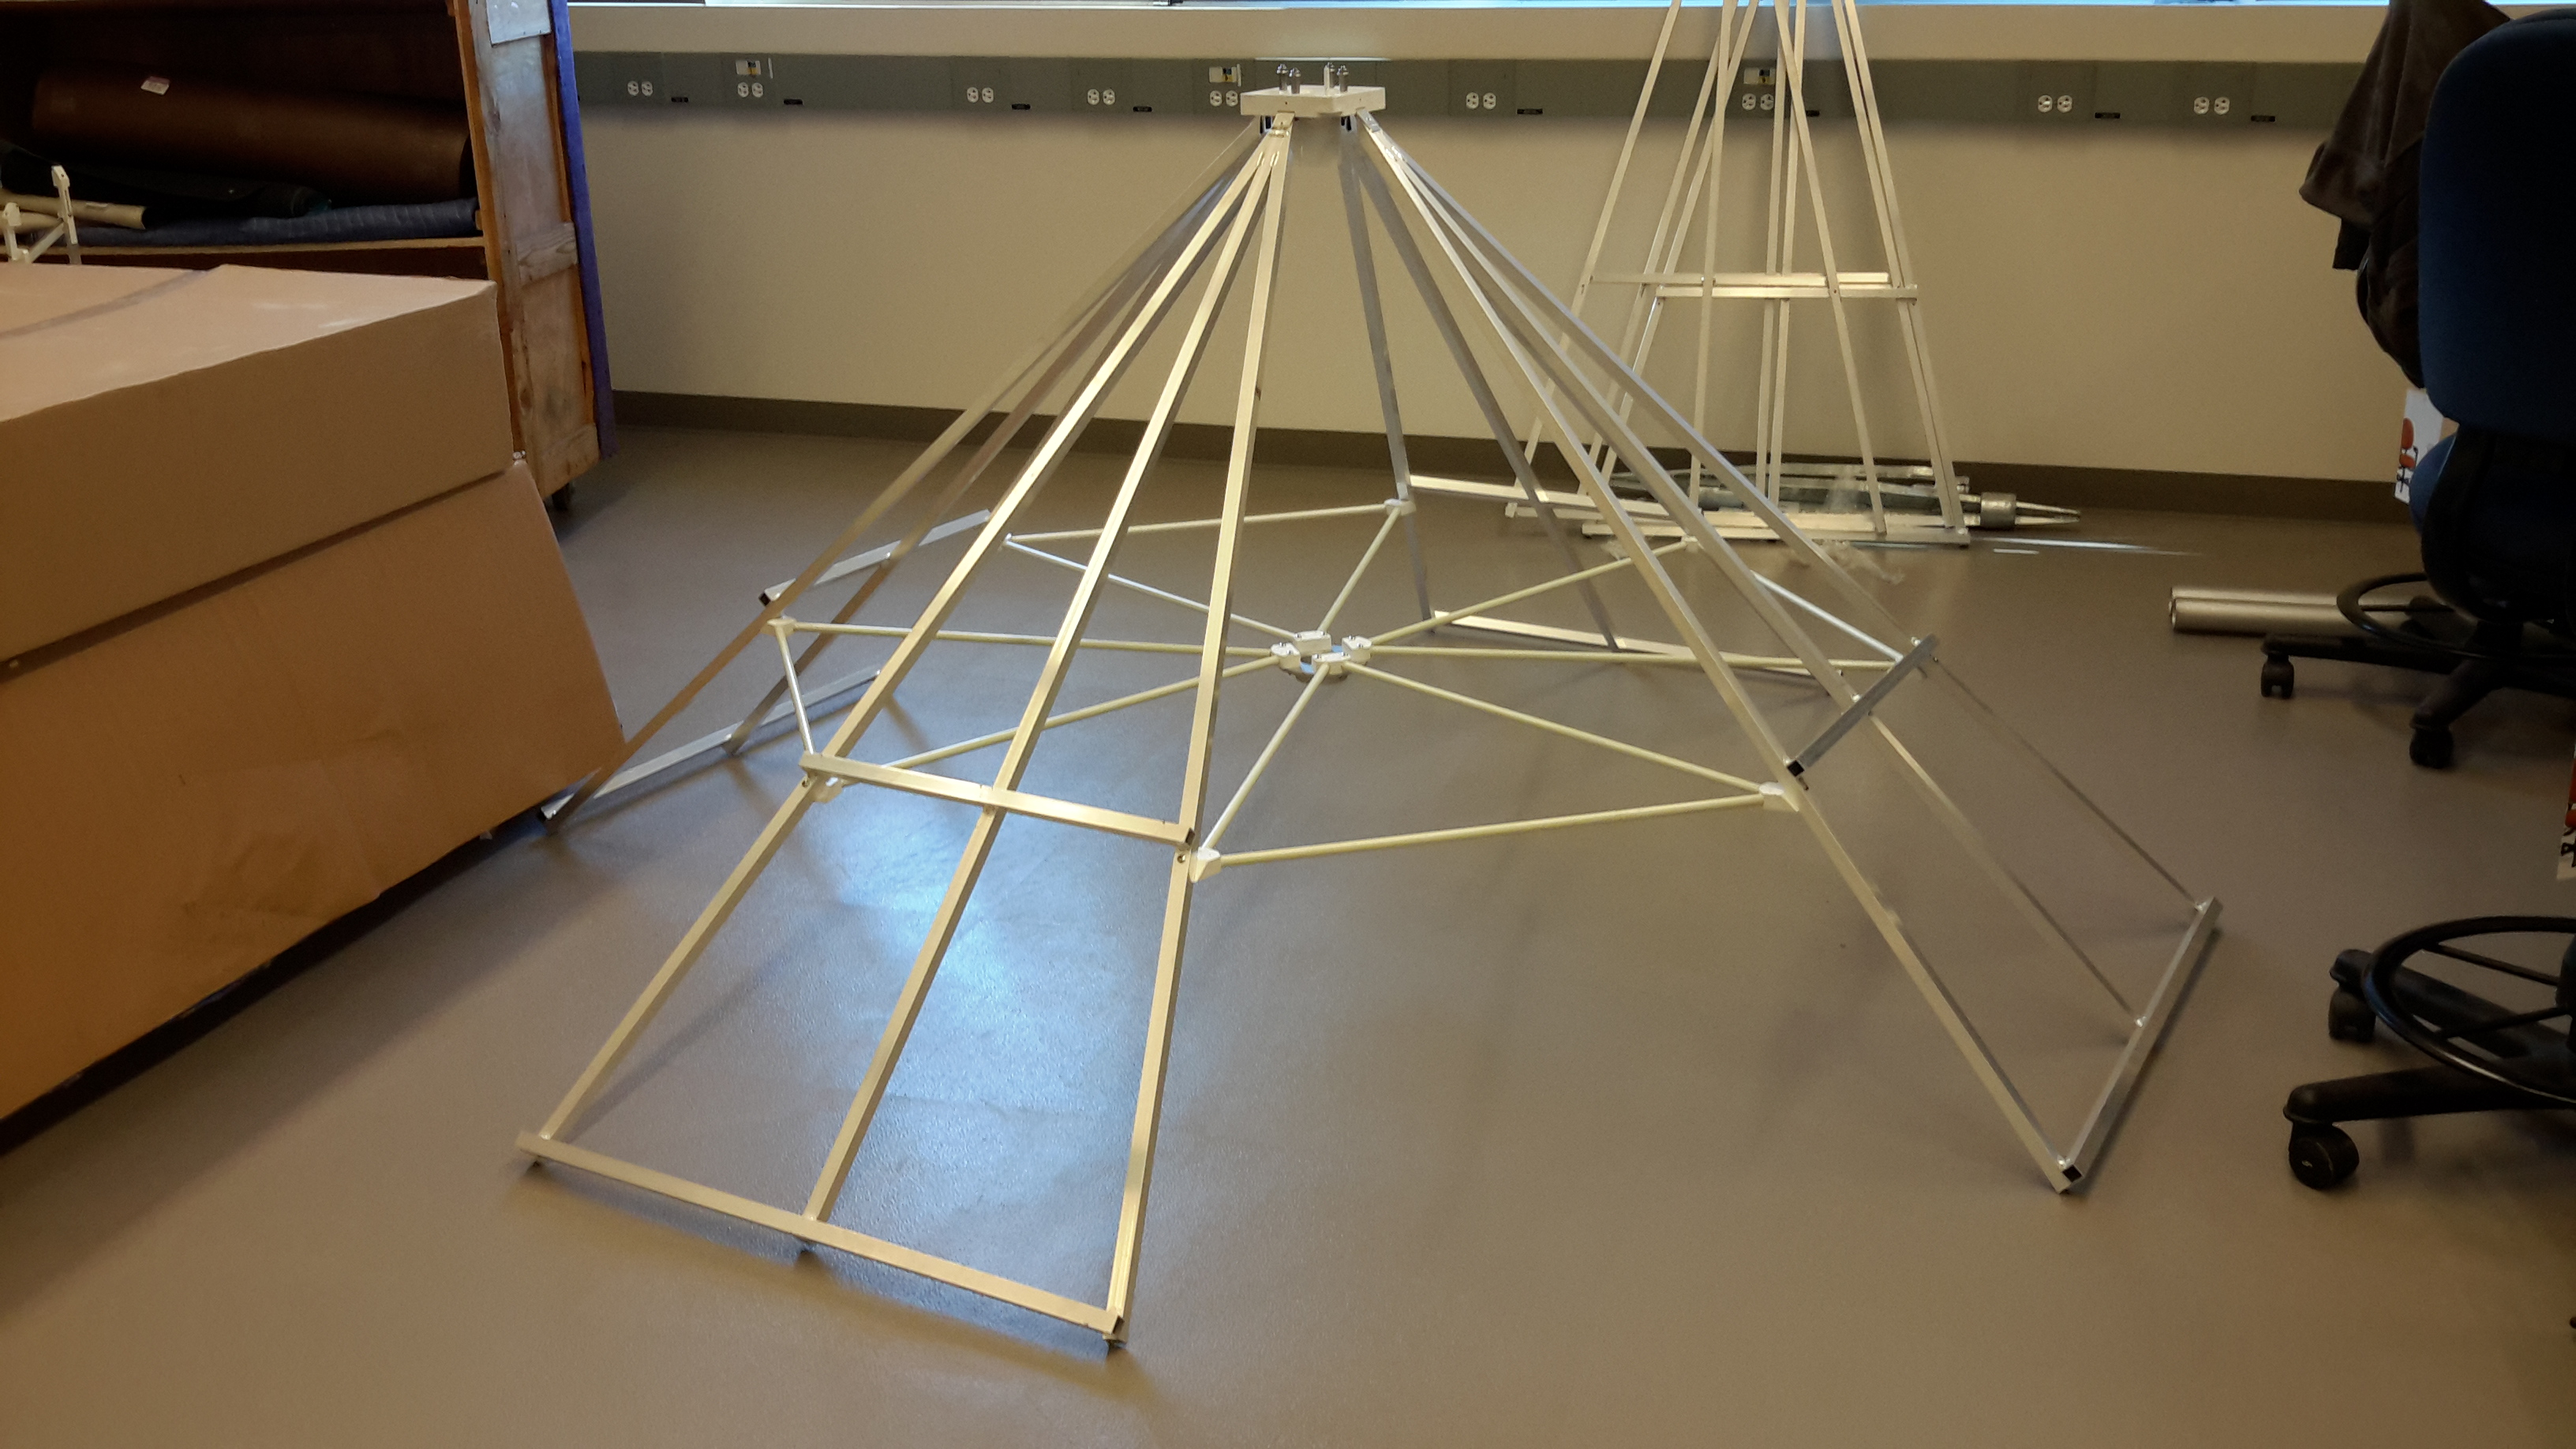
\includegraphics[width=\linewidth]{plots/20141125_112538.jpg}
	\caption{Element with triangle assembly and hub attached. \label{AlmostCompleteElement}}
\end{figure}
			
\end{enumerate}
\end{document}
